\documentclass[twoside]{book}

% Packages required by doxygen
\usepackage{fixltx2e}
\usepackage{calc}
\usepackage{doxygen}
\usepackage[export]{adjustbox} % also loads graphicx
\usepackage{graphicx}
\usepackage[utf8]{inputenc}
\usepackage{makeidx}
\usepackage{multicol}
\usepackage{multirow}
\PassOptionsToPackage{warn}{textcomp}
\usepackage{textcomp}
\usepackage[nointegrals]{wasysym}
\usepackage[table]{xcolor}

% Font selection
\usepackage[T1]{fontenc}
\usepackage[scaled=.90]{helvet}
\usepackage{courier}
\usepackage{amssymb}
\usepackage{sectsty}
\renewcommand{\familydefault}{\sfdefault}
\allsectionsfont{%
  \fontseries{bc}\selectfont%
  \color{darkgray}%
}
\renewcommand{\DoxyLabelFont}{%
  \fontseries{bc}\selectfont%
  \color{darkgray}%
}
\newcommand{\+}{\discretionary{\mbox{\scriptsize$\hookleftarrow$}}{}{}}

% Page & text layout
\usepackage{geometry}
\geometry{%
  a4paper,%
  top=2.5cm,%
  bottom=2.5cm,%
  left=2.5cm,%
  right=2.5cm%
}
\tolerance=750
\hfuzz=15pt
\hbadness=750
\setlength{\emergencystretch}{15pt}
\setlength{\parindent}{0cm}
\setlength{\parskip}{3ex plus 2ex minus 2ex}
\makeatletter
\renewcommand{\paragraph}{%
  \@startsection{paragraph}{4}{0ex}{-1.0ex}{1.0ex}{%
    \normalfont\normalsize\bfseries\SS@parafont%
  }%
}
\renewcommand{\subparagraph}{%
  \@startsection{subparagraph}{5}{0ex}{-1.0ex}{1.0ex}{%
    \normalfont\normalsize\bfseries\SS@subparafont%
  }%
}
\makeatother

% Headers & footers
\usepackage{fancyhdr}
\pagestyle{fancyplain}
\fancyhead[LE]{\fancyplain{}{\bfseries\thepage}}
\fancyhead[CE]{\fancyplain{}{}}
\fancyhead[RE]{\fancyplain{}{\bfseries\leftmark}}
\fancyhead[LO]{\fancyplain{}{\bfseries\rightmark}}
\fancyhead[CO]{\fancyplain{}{}}
\fancyhead[RO]{\fancyplain{}{\bfseries\thepage}}
\fancyfoot[LE]{\fancyplain{}{}}
\fancyfoot[CE]{\fancyplain{}{}}
\fancyfoot[RE]{\fancyplain{}{\bfseries\scriptsize Generated by Doxygen }}
\fancyfoot[LO]{\fancyplain{}{\bfseries\scriptsize Generated by Doxygen }}
\fancyfoot[CO]{\fancyplain{}{}}
\fancyfoot[RO]{\fancyplain{}{}}
\renewcommand{\footrulewidth}{0.4pt}
\renewcommand{\chaptermark}[1]{%
  \markboth{#1}{}%
}
\renewcommand{\sectionmark}[1]{%
  \markright{\thesection\ #1}%
}

% Indices & bibliography
\usepackage{natbib}
\usepackage[titles]{tocloft}
\setcounter{tocdepth}{3}
\setcounter{secnumdepth}{5}
\makeindex

% Hyperlinks (required, but should be loaded last)
\usepackage{ifpdf}
\ifpdf
  \usepackage[pdftex,pagebackref=true]{hyperref}
\else
  \usepackage[ps2pdf,pagebackref=true]{hyperref}
\fi
\hypersetup{%
  colorlinks=true,%
  linkcolor=blue,%
  citecolor=blue,%
  unicode%
}

% Custom commands
\newcommand{\clearemptydoublepage}{%
  \newpage{\pagestyle{empty}\cleardoublepage}%
}

\usepackage{caption}
\captionsetup{labelsep=space,justification=centering,font={bf},singlelinecheck=off,skip=4pt,position=top}

%===== C O N T E N T S =====

\begin{document}

% Titlepage & ToC
\hypersetup{pageanchor=false,
             bookmarksnumbered=true,
             pdfencoding=unicode
            }
\pagenumbering{roman}
\begin{titlepage}
\vspace*{7cm}
\begin{center}%
{\Large U\+O\+RA simulation and analysis }\\
\vspace*{1cm}
{\large Generated by Doxygen 1.8.11}\\
\end{center}
\end{titlepage}
\clearemptydoublepage
\tableofcontents
\clearemptydoublepage
\pagenumbering{arabic}
\hypersetup{pageanchor=true}

%--- Begin generated contents ---
\chapter{File Index}
\section{File List}
Here is a list of all files with brief descriptions\+:\begin{DoxyCompactList}
\item\contentsline{section}{\hyperlink{dynamic__analysis_8c}{dynamic\+\_\+analysis.\+c} \\*Dynamic analysis }{\pageref{dd/d14/dynamic__analysis_8c}}{}
\item\contentsline{section}{\hyperlink{dynamic__simulation__R_8c}{dynamic\+\_\+simulation\+\_\+\+R.\+c} }{\pageref{d2/d2a/dynamic__simulation__R_8c}}{}
\end{DoxyCompactList}

\chapter{File Documentation}
\hypertarget{dynamic__analysis_8c}{}\section{dynamic\+\_\+analysis.\+c File Reference}
\label{dynamic__analysis_8c}\index{dynamic\+\_\+analysis.\+c@{dynamic\+\_\+analysis.\+c}}


dynamic analysis  


{\ttfamily \#include $<$stdio.\+h$>$}\\*
{\ttfamily \#include $<$stdlib.\+h$>$}\\*
{\ttfamily \#include $<$math.\+h$>$}\\*
{\ttfamily \#include $<$time.\+h$>$}\\*
Include dependency graph for dynamic\+\_\+analysis.\+c\+:\nopagebreak
\begin{figure}[H]
\begin{center}
\leavevmode
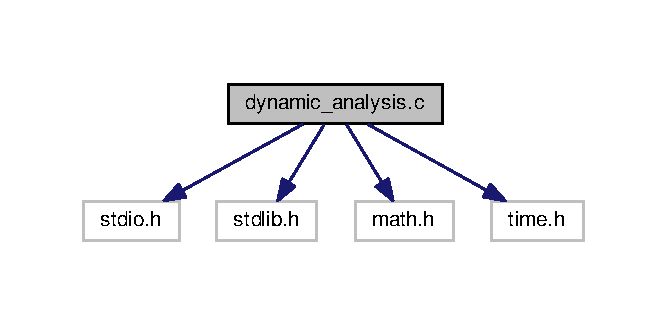
\includegraphics[width=320pt]{df/dc2/dynamic__analysis_8c__incl}
\end{center}
\end{figure}
\subsection*{Functions}
\begin{DoxyCompactItemize}
\item 
int \hyperlink{dynamic__analysis_8c_a44c532972eac9a2be87f26f5f9a171a1}{station\+\_\+number} ()
\begin{DoxyCompactList}\small\item\em for calculating the number of success S\+TA, and performance metrics \end{DoxyCompactList}\item 
int \hyperlink{dynamic__analysis_8c_ae66f6b31b5ad750f1fe042a706a4e3d4}{main} ()
\end{DoxyCompactItemize}
\subsection*{Variables}
\begin{DoxyCompactItemize}
\item 
int \hyperlink{dynamic__analysis_8c_ab2cb8ab426f06c27553b10c73a4f795c}{sta} = 40
\begin{DoxyCompactList}\small\item\em parameter definition \end{DoxyCompactList}\item 
int \hyperlink{dynamic__analysis_8c_a66220f2712ab879767e2b0b1f3e79c1d}{Lmax} = 5
\begin{DoxyCompactList}\small\item\em retry limit \end{DoxyCompactList}\item 
int \hyperlink{dynamic__analysis_8c_a504e9c4516d3b4089e4a9ea17c2ef2fa}{Imax} = 34
\begin{DoxyCompactList}\small\item\em Imax. \end{DoxyCompactList}\item 
float \hyperlink{dynamic__analysis_8c_ae93883d7b7e696e378c6816f9f77b037}{T\+X\+OP} = 5.\+681
\begin{DoxyCompactList}\small\item\em The length of T\+X\+OP. \end{DoxyCompactList}\item 
int \hyperlink{dynamic__analysis_8c_aa1ce3a5eea7d7c9e58a5755bf12e0510}{Jmax}
\begin{DoxyCompactList}\small\item\em maximum J \end{DoxyCompactList}\item 
int \hyperlink{dynamic__analysis_8c_a28b532b3cf29162409a495ecf16c4efd}{Jmin}
\begin{DoxyCompactList}\small\item\em minimum J \end{DoxyCompactList}\item 
float \hyperlink{dynamic__analysis_8c_ae5acbf81614d055ed8075397f98f9493}{a\+\_\+j\+\_\+i}
\begin{DoxyCompactList}\small\item\em alpha\+\_\+j\+\_\+i \end{DoxyCompactList}\item 
int \hyperlink{dynamic__analysis_8c_a3d90133d3051fbc4816d02efd9566d8e}{R} = 15
\begin{DoxyCompactList}\small\item\em RU. \end{DoxyCompactList}\item 
int \hyperlink{dynamic__analysis_8c_a2689c4b3931025b79053532a5f1b0a85}{K} = 10
\begin{DoxyCompactList}\small\item\em reserved slots \end{DoxyCompactList}\item 
int \hyperlink{dynamic__analysis_8c_a1dfcb70b9229f2da17dd5922b87ecf2c}{delta} = 0
\begin{DoxyCompactList}\small\item\em delta \end{DoxyCompactList}\item 
float \hyperlink{dynamic__analysis_8c_a1a86abc0e3b72c599d11f8fca1fe029b}{Ri} \mbox{[}100\mbox{]}
\begin{DoxyCompactList}\small\item\em number of R\+A-\/\+RU in ith slot \end{DoxyCompactList}\item 
float \hyperlink{dynamic__analysis_8c_a28e79d928b8e2e20d0836b652f98ea46}{total\+\_\+\+Ri}
\item 
int \hyperlink{dynamic__analysis_8c_acb559820d9ca11295b4500f179ef6392}{i}
\begin{DoxyCompactList}\small\item\em index of for loop \end{DoxyCompactList}\item 
int \hyperlink{dynamic__analysis_8c_ab66ed8e0098c0a86b458672a55a9cca9}{k}
\begin{DoxyCompactList}\small\item\em index of for loop \end{DoxyCompactList}\item 
int \hyperlink{dynamic__analysis_8c_a76f11d9a0a47b94f72c2d0e77fb32240}{n}
\begin{DoxyCompactList}\small\item\em index of for loop \end{DoxyCompactList}\item 
int \hyperlink{dynamic__analysis_8c_a742204794ea328ba293fe59cec79b990}{m}
\begin{DoxyCompactList}\small\item\em index of for loop \end{DoxyCompactList}\item 
int \hyperlink{dynamic__analysis_8c_a4e1e0e72dd773439e333c84dd762a9c3}{c}
\begin{DoxyCompactList}\small\item\em index of for loop \end{DoxyCompactList}\item 
int \hyperlink{dynamic__analysis_8c_a7bfb4915d0ef30a664c014be00bad1fe}{Nn}
\item 
int \hyperlink{dynamic__analysis_8c_a37d972ae0b47b9099e30983131d31916}{j}
\item 
int \hyperlink{dynamic__analysis_8c_a9dc38bd3fb41a39752550015ef4f512c}{Nn\+\_\+index}
\item 
int \hyperlink{dynamic__analysis_8c_aa4c2a5552e9bc49b1816ff532f558c74}{a}
\item 
float \hyperlink{dynamic__analysis_8c_aeeafe7e9eebbd2a45ce4fa2ae0d96c51}{sum}
\begin{DoxyCompactList}\small\item\em temp for calculating Imax \end{DoxyCompactList}\item 
float \hyperlink{dynamic__analysis_8c_a24d61a35b72d7299eb6b5f48e71a571b}{temp}
\item 
float \hyperlink{dynamic__analysis_8c_a5e005e112ca8edcc1d9b59fdfaefb7fd}{temp1}
\item 
double \hyperlink{dynamic__analysis_8c_a6770f4b277df418aa6ed32716aabc69b}{access\+\_\+delay}
\begin{DoxyCompactList}\small\item\em for access delay \end{DoxyCompactList}\item 
double \hyperlink{dynamic__analysis_8c_a15c142af1b2266dbf4bcf5cf69516be1}{counter\+\_\+access\+\_\+delay}
\begin{DoxyCompactList}\small\item\em for access delay \end{DoxyCompactList}\item 
double \hyperlink{dynamic__analysis_8c_a8390a777ee84b713b09fcbb5d2f47024}{Fm} \mbox{[}6\mbox{]}
\begin{DoxyCompactList}\small\item\em for C\+DF \end{DoxyCompactList}\item 
double \hyperlink{dynamic__analysis_8c_af1cb1a10f88721b26875206ca5f93b92}{total\+\_\+cdf}
\begin{DoxyCompactList}\small\item\em for C\+DF \end{DoxyCompactList}\item 
double \hyperlink{dynamic__analysis_8c_a6f488533feeb78b1a439a47fafc6420b}{final\+\_\+cdf}
\begin{DoxyCompactList}\small\item\em for C\+DF \end{DoxyCompactList}\item 
int \hyperlink{dynamic__analysis_8c_a19c303b09c0b5fda03eba722a14650c1}{O\+CW} \mbox{[}16\mbox{]}
\begin{DoxyCompactList}\small\item\em O\+C\+Wn. \end{DoxyCompactList}\item 
double \hyperlink{dynamic__analysis_8c_a345c2951b3e156ffc738e0de807642b4}{success\+\_\+sta}
\begin{DoxyCompactList}\small\item\em for success S\+TA, packet \end{DoxyCompactList}\item 
double \hyperlink{dynamic__analysis_8c_aa432b6257e899272f50f3ced74d4268e}{success\+\_\+packet}
\begin{DoxyCompactList}\small\item\em for success packet \end{DoxyCompactList}\item 
float \hyperlink{dynamic__analysis_8c_a3ebded876cc18042b8855cd4c27c00ae}{R\+A\+\_\+\+RU} = 15.\+0
\begin{DoxyCompactList}\small\item\em R\+A-\/\+RU in first slot. \end{DoxyCompactList}\item 
double \hyperlink{dynamic__analysis_8c_a468749690692c0379578a882d18ae03f}{M} \mbox{[}100\mbox{]}
\begin{DoxyCompactList}\small\item\em array for M \end{DoxyCompactList}\item 
double \hyperlink{dynamic__analysis_8c_ae543cde0580d71ac9500d7b81128d3f2}{M\+\_\+i} \mbox{[}100\mbox{]}\mbox{[}6\mbox{]}
\begin{DoxyCompactList}\small\item\em array for Mi \end{DoxyCompactList}\item 
double \hyperlink{dynamic__analysis_8c_a4bd37829ebbeaeb19ae8018f49a33ec9}{M\+\_\+i\+\_\+s} \mbox{[}100\mbox{]}\mbox{[}6\mbox{]}
\begin{DoxyCompactList}\small\item\em array for Mis \end{DoxyCompactList}\item 
double \hyperlink{dynamic__analysis_8c_a0598245ad000ad15390cb80d45ea2252}{M\+\_\+i\+\_\+f} \mbox{[}100\mbox{]}\mbox{[}6\mbox{]}
\begin{DoxyCompactList}\small\item\em array for Mif \end{DoxyCompactList}\item 
double \hyperlink{dynamic__analysis_8c_a49abb259b07d52a183751e5401ee8594}{M\+\_\+i\+\_\+s\+\_\+C} \mbox{[}100\mbox{]}
\begin{DoxyCompactList}\small\item\em array for MisC \end{DoxyCompactList}\item 
double \hyperlink{dynamic__analysis_8c_a621ed640a0caba2d42ecb9b7d376b3f0}{success\+\_\+probability}
\begin{DoxyCompactList}\small\item\em access success probability \end{DoxyCompactList}\end{DoxyCompactItemize}


\subsection{Detailed Description}
dynamic analysis 



\subsection{Function Documentation}
\index{dynamic\+\_\+analysis.\+c@{dynamic\+\_\+analysis.\+c}!main@{main}}
\index{main@{main}!dynamic\+\_\+analysis.\+c@{dynamic\+\_\+analysis.\+c}}
\subsubsection[{\texorpdfstring{main()}{main()}}]{\setlength{\rightskip}{0pt plus 5cm}int main (
\begin{DoxyParamCaption}
{}
\end{DoxyParamCaption}
)}\hypertarget{dynamic__analysis_8c_ae66f6b31b5ad750f1fe042a706a4e3d4}{}\label{dynamic__analysis_8c_ae66f6b31b5ad750f1fe042a706a4e3d4}


References station\+\_\+number().



Here is the call graph for this function\+:\nopagebreak
\begin{figure}[H]
\begin{center}
\leavevmode
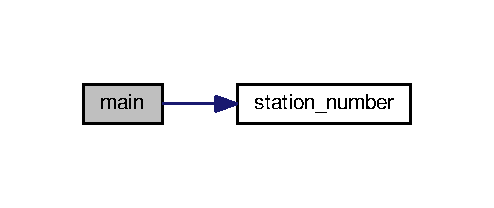
\includegraphics[width=237pt]{dd/d14/dynamic__analysis_8c_ae66f6b31b5ad750f1fe042a706a4e3d4_cgraph}
\end{center}
\end{figure}


\index{dynamic\+\_\+analysis.\+c@{dynamic\+\_\+analysis.\+c}!station\+\_\+number@{station\+\_\+number}}
\index{station\+\_\+number@{station\+\_\+number}!dynamic\+\_\+analysis.\+c@{dynamic\+\_\+analysis.\+c}}
\subsubsection[{\texorpdfstring{station\+\_\+number()}{station_number()}}]{\setlength{\rightskip}{0pt plus 5cm}int station\+\_\+number (
\begin{DoxyParamCaption}
{}
\end{DoxyParamCaption}
)}\hypertarget{dynamic__analysis_8c_a44c532972eac9a2be87f26f5f9a171a1}{}\label{dynamic__analysis_8c_a44c532972eac9a2be87f26f5f9a171a1}


for calculating the number of success S\+TA, and performance metrics 

Ri = Ri-\/1 -\/ Mi-\/1,s + Mi-\/K,s

Ri for delta

min(2$\ast$\+O\+C\+W+1,O\+C\+Wmax)

initial condition

Mi\mbox{[}n\mbox{]}=sigma (a\+\_\+j\+\_\+i$\ast$\+Mj,F\mbox{[}n-\/1\mbox{]})

statistics

performance metric

success probability

access delay

C\+DF

i v.\+s. M\+\_\+i,s\mbox{[}n\mbox{]}

Imax 

References a\+\_\+j\+\_\+i, access\+\_\+delay, c, counter\+\_\+access\+\_\+delay, delta, final\+\_\+cdf, Fm, i, Imax, K, k, Lmax, m, M, M\+\_\+i, M\+\_\+i\+\_\+f, M\+\_\+i\+\_\+s, M\+\_\+i\+\_\+s\+\_\+C, n, Nn, Nn\+\_\+index, O\+CW, R\+A\+\_\+\+RU, Ri, sta, success\+\_\+packet, success\+\_\+probability, success\+\_\+sta, sum, temp, temp1, total\+\_\+cdf, and T\+X\+OP.



Referenced by main().



\subsection{Variable Documentation}
\index{dynamic\+\_\+analysis.\+c@{dynamic\+\_\+analysis.\+c}!a@{a}}
\index{a@{a}!dynamic\+\_\+analysis.\+c@{dynamic\+\_\+analysis.\+c}}
\subsubsection[{\texorpdfstring{a}{a}}]{\setlength{\rightskip}{0pt plus 5cm}int a}\hypertarget{dynamic__analysis_8c_aa4c2a5552e9bc49b1816ff532f558c74}{}\label{dynamic__analysis_8c_aa4c2a5552e9bc49b1816ff532f558c74}
\index{dynamic\+\_\+analysis.\+c@{dynamic\+\_\+analysis.\+c}!a\+\_\+j\+\_\+i@{a\+\_\+j\+\_\+i}}
\index{a\+\_\+j\+\_\+i@{a\+\_\+j\+\_\+i}!dynamic\+\_\+analysis.\+c@{dynamic\+\_\+analysis.\+c}}
\subsubsection[{\texorpdfstring{a\+\_\+j\+\_\+i}{a_j_i}}]{\setlength{\rightskip}{0pt plus 5cm}float a\+\_\+j\+\_\+i}\hypertarget{dynamic__analysis_8c_ae5acbf81614d055ed8075397f98f9493}{}\label{dynamic__analysis_8c_ae5acbf81614d055ed8075397f98f9493}


alpha\+\_\+j\+\_\+i 



Referenced by station\+\_\+number().

\index{dynamic\+\_\+analysis.\+c@{dynamic\+\_\+analysis.\+c}!access\+\_\+delay@{access\+\_\+delay}}
\index{access\+\_\+delay@{access\+\_\+delay}!dynamic\+\_\+analysis.\+c@{dynamic\+\_\+analysis.\+c}}
\subsubsection[{\texorpdfstring{access\+\_\+delay}{access_delay}}]{\setlength{\rightskip}{0pt plus 5cm}double access\+\_\+delay}\hypertarget{dynamic__analysis_8c_a6770f4b277df418aa6ed32716aabc69b}{}\label{dynamic__analysis_8c_a6770f4b277df418aa6ed32716aabc69b}


for access delay 



Referenced by station\+\_\+number().

\index{dynamic\+\_\+analysis.\+c@{dynamic\+\_\+analysis.\+c}!c@{c}}
\index{c@{c}!dynamic\+\_\+analysis.\+c@{dynamic\+\_\+analysis.\+c}}
\subsubsection[{\texorpdfstring{c}{c}}]{\setlength{\rightskip}{0pt plus 5cm}int c}\hypertarget{dynamic__analysis_8c_a4e1e0e72dd773439e333c84dd762a9c3}{}\label{dynamic__analysis_8c_a4e1e0e72dd773439e333c84dd762a9c3}


index of for loop 



Referenced by station\+\_\+number().

\index{dynamic\+\_\+analysis.\+c@{dynamic\+\_\+analysis.\+c}!counter\+\_\+access\+\_\+delay@{counter\+\_\+access\+\_\+delay}}
\index{counter\+\_\+access\+\_\+delay@{counter\+\_\+access\+\_\+delay}!dynamic\+\_\+analysis.\+c@{dynamic\+\_\+analysis.\+c}}
\subsubsection[{\texorpdfstring{counter\+\_\+access\+\_\+delay}{counter_access_delay}}]{\setlength{\rightskip}{0pt plus 5cm}double counter\+\_\+access\+\_\+delay}\hypertarget{dynamic__analysis_8c_a15c142af1b2266dbf4bcf5cf69516be1}{}\label{dynamic__analysis_8c_a15c142af1b2266dbf4bcf5cf69516be1}


for access delay 



Referenced by station\+\_\+number().

\index{dynamic\+\_\+analysis.\+c@{dynamic\+\_\+analysis.\+c}!delta@{delta}}
\index{delta@{delta}!dynamic\+\_\+analysis.\+c@{dynamic\+\_\+analysis.\+c}}
\subsubsection[{\texorpdfstring{delta}{delta}}]{\setlength{\rightskip}{0pt plus 5cm}int delta = 0}\hypertarget{dynamic__analysis_8c_a1dfcb70b9229f2da17dd5922b87ecf2c}{}\label{dynamic__analysis_8c_a1dfcb70b9229f2da17dd5922b87ecf2c}


delta 



Referenced by station\+\_\+number().

\index{dynamic\+\_\+analysis.\+c@{dynamic\+\_\+analysis.\+c}!final\+\_\+cdf@{final\+\_\+cdf}}
\index{final\+\_\+cdf@{final\+\_\+cdf}!dynamic\+\_\+analysis.\+c@{dynamic\+\_\+analysis.\+c}}
\subsubsection[{\texorpdfstring{final\+\_\+cdf}{final_cdf}}]{\setlength{\rightskip}{0pt plus 5cm}double final\+\_\+cdf}\hypertarget{dynamic__analysis_8c_a6f488533feeb78b1a439a47fafc6420b}{}\label{dynamic__analysis_8c_a6f488533feeb78b1a439a47fafc6420b}


for C\+DF 



Referenced by station\+\_\+number().

\index{dynamic\+\_\+analysis.\+c@{dynamic\+\_\+analysis.\+c}!Fm@{Fm}}
\index{Fm@{Fm}!dynamic\+\_\+analysis.\+c@{dynamic\+\_\+analysis.\+c}}
\subsubsection[{\texorpdfstring{Fm}{Fm}}]{\setlength{\rightskip}{0pt plus 5cm}double Fm\mbox{[}6\mbox{]}}\hypertarget{dynamic__analysis_8c_a8390a777ee84b713b09fcbb5d2f47024}{}\label{dynamic__analysis_8c_a8390a777ee84b713b09fcbb5d2f47024}


for C\+DF 



Referenced by station\+\_\+number().

\index{dynamic\+\_\+analysis.\+c@{dynamic\+\_\+analysis.\+c}!i@{i}}
\index{i@{i}!dynamic\+\_\+analysis.\+c@{dynamic\+\_\+analysis.\+c}}
\subsubsection[{\texorpdfstring{i}{i}}]{\setlength{\rightskip}{0pt plus 5cm}int i}\hypertarget{dynamic__analysis_8c_acb559820d9ca11295b4500f179ef6392}{}\label{dynamic__analysis_8c_acb559820d9ca11295b4500f179ef6392}


index of for loop 



Referenced by station\+\_\+number().

\index{dynamic\+\_\+analysis.\+c@{dynamic\+\_\+analysis.\+c}!Imax@{Imax}}
\index{Imax@{Imax}!dynamic\+\_\+analysis.\+c@{dynamic\+\_\+analysis.\+c}}
\subsubsection[{\texorpdfstring{Imax}{Imax}}]{\setlength{\rightskip}{0pt plus 5cm}int Imax = 34}\hypertarget{dynamic__analysis_8c_a504e9c4516d3b4089e4a9ea17c2ef2fa}{}\label{dynamic__analysis_8c_a504e9c4516d3b4089e4a9ea17c2ef2fa}


Imax. 



Referenced by station\+\_\+number().

\index{dynamic\+\_\+analysis.\+c@{dynamic\+\_\+analysis.\+c}!j@{j}}
\index{j@{j}!dynamic\+\_\+analysis.\+c@{dynamic\+\_\+analysis.\+c}}
\subsubsection[{\texorpdfstring{j}{j}}]{\setlength{\rightskip}{0pt plus 5cm}int j}\hypertarget{dynamic__analysis_8c_a37d972ae0b47b9099e30983131d31916}{}\label{dynamic__analysis_8c_a37d972ae0b47b9099e30983131d31916}
\index{dynamic\+\_\+analysis.\+c@{dynamic\+\_\+analysis.\+c}!Jmax@{Jmax}}
\index{Jmax@{Jmax}!dynamic\+\_\+analysis.\+c@{dynamic\+\_\+analysis.\+c}}
\subsubsection[{\texorpdfstring{Jmax}{Jmax}}]{\setlength{\rightskip}{0pt plus 5cm}int Jmax}\hypertarget{dynamic__analysis_8c_aa1ce3a5eea7d7c9e58a5755bf12e0510}{}\label{dynamic__analysis_8c_aa1ce3a5eea7d7c9e58a5755bf12e0510}


maximum J 

\index{dynamic\+\_\+analysis.\+c@{dynamic\+\_\+analysis.\+c}!Jmin@{Jmin}}
\index{Jmin@{Jmin}!dynamic\+\_\+analysis.\+c@{dynamic\+\_\+analysis.\+c}}
\subsubsection[{\texorpdfstring{Jmin}{Jmin}}]{\setlength{\rightskip}{0pt plus 5cm}int Jmin}\hypertarget{dynamic__analysis_8c_a28b532b3cf29162409a495ecf16c4efd}{}\label{dynamic__analysis_8c_a28b532b3cf29162409a495ecf16c4efd}


minimum J 

\index{dynamic\+\_\+analysis.\+c@{dynamic\+\_\+analysis.\+c}!K@{K}}
\index{K@{K}!dynamic\+\_\+analysis.\+c@{dynamic\+\_\+analysis.\+c}}
\subsubsection[{\texorpdfstring{K}{K}}]{\setlength{\rightskip}{0pt plus 5cm}int K = 10}\hypertarget{dynamic__analysis_8c_a2689c4b3931025b79053532a5f1b0a85}{}\label{dynamic__analysis_8c_a2689c4b3931025b79053532a5f1b0a85}


reserved slots 



Referenced by station\+\_\+number().

\index{dynamic\+\_\+analysis.\+c@{dynamic\+\_\+analysis.\+c}!k@{k}}
\index{k@{k}!dynamic\+\_\+analysis.\+c@{dynamic\+\_\+analysis.\+c}}
\subsubsection[{\texorpdfstring{k}{k}}]{\setlength{\rightskip}{0pt plus 5cm}int k}\hypertarget{dynamic__analysis_8c_ab66ed8e0098c0a86b458672a55a9cca9}{}\label{dynamic__analysis_8c_ab66ed8e0098c0a86b458672a55a9cca9}


index of for loop 



Referenced by station\+\_\+number().

\index{dynamic\+\_\+analysis.\+c@{dynamic\+\_\+analysis.\+c}!Lmax@{Lmax}}
\index{Lmax@{Lmax}!dynamic\+\_\+analysis.\+c@{dynamic\+\_\+analysis.\+c}}
\subsubsection[{\texorpdfstring{Lmax}{Lmax}}]{\setlength{\rightskip}{0pt plus 5cm}int Lmax = 5}\hypertarget{dynamic__analysis_8c_a66220f2712ab879767e2b0b1f3e79c1d}{}\label{dynamic__analysis_8c_a66220f2712ab879767e2b0b1f3e79c1d}


retry limit 



Referenced by station\+\_\+number().

\index{dynamic\+\_\+analysis.\+c@{dynamic\+\_\+analysis.\+c}!m@{m}}
\index{m@{m}!dynamic\+\_\+analysis.\+c@{dynamic\+\_\+analysis.\+c}}
\subsubsection[{\texorpdfstring{m}{m}}]{\setlength{\rightskip}{0pt plus 5cm}int m}\hypertarget{dynamic__analysis_8c_a742204794ea328ba293fe59cec79b990}{}\label{dynamic__analysis_8c_a742204794ea328ba293fe59cec79b990}


index of for loop 



Referenced by station\+\_\+number().

\index{dynamic\+\_\+analysis.\+c@{dynamic\+\_\+analysis.\+c}!M@{M}}
\index{M@{M}!dynamic\+\_\+analysis.\+c@{dynamic\+\_\+analysis.\+c}}
\subsubsection[{\texorpdfstring{M}{M}}]{\setlength{\rightskip}{0pt plus 5cm}double M\mbox{[}100\mbox{]}}\hypertarget{dynamic__analysis_8c_a468749690692c0379578a882d18ae03f}{}\label{dynamic__analysis_8c_a468749690692c0379578a882d18ae03f}


array for M 



Referenced by station\+\_\+number().

\index{dynamic\+\_\+analysis.\+c@{dynamic\+\_\+analysis.\+c}!M\+\_\+i@{M\+\_\+i}}
\index{M\+\_\+i@{M\+\_\+i}!dynamic\+\_\+analysis.\+c@{dynamic\+\_\+analysis.\+c}}
\subsubsection[{\texorpdfstring{M\+\_\+i}{M_i}}]{\setlength{\rightskip}{0pt plus 5cm}double M\+\_\+i\mbox{[}100\mbox{]}\mbox{[}6\mbox{]}}\hypertarget{dynamic__analysis_8c_ae543cde0580d71ac9500d7b81128d3f2}{}\label{dynamic__analysis_8c_ae543cde0580d71ac9500d7b81128d3f2}


array for Mi 



Referenced by station\+\_\+number().

\index{dynamic\+\_\+analysis.\+c@{dynamic\+\_\+analysis.\+c}!M\+\_\+i\+\_\+f@{M\+\_\+i\+\_\+f}}
\index{M\+\_\+i\+\_\+f@{M\+\_\+i\+\_\+f}!dynamic\+\_\+analysis.\+c@{dynamic\+\_\+analysis.\+c}}
\subsubsection[{\texorpdfstring{M\+\_\+i\+\_\+f}{M_i_f}}]{\setlength{\rightskip}{0pt plus 5cm}double M\+\_\+i\+\_\+f\mbox{[}100\mbox{]}\mbox{[}6\mbox{]}}\hypertarget{dynamic__analysis_8c_a0598245ad000ad15390cb80d45ea2252}{}\label{dynamic__analysis_8c_a0598245ad000ad15390cb80d45ea2252}


array for Mif 



Referenced by station\+\_\+number().

\index{dynamic\+\_\+analysis.\+c@{dynamic\+\_\+analysis.\+c}!M\+\_\+i\+\_\+s@{M\+\_\+i\+\_\+s}}
\index{M\+\_\+i\+\_\+s@{M\+\_\+i\+\_\+s}!dynamic\+\_\+analysis.\+c@{dynamic\+\_\+analysis.\+c}}
\subsubsection[{\texorpdfstring{M\+\_\+i\+\_\+s}{M_i_s}}]{\setlength{\rightskip}{0pt plus 5cm}double M\+\_\+i\+\_\+s\mbox{[}100\mbox{]}\mbox{[}6\mbox{]}}\hypertarget{dynamic__analysis_8c_a4bd37829ebbeaeb19ae8018f49a33ec9}{}\label{dynamic__analysis_8c_a4bd37829ebbeaeb19ae8018f49a33ec9}


array for Mis 



Referenced by station\+\_\+number().

\index{dynamic\+\_\+analysis.\+c@{dynamic\+\_\+analysis.\+c}!M\+\_\+i\+\_\+s\+\_\+C@{M\+\_\+i\+\_\+s\+\_\+C}}
\index{M\+\_\+i\+\_\+s\+\_\+C@{M\+\_\+i\+\_\+s\+\_\+C}!dynamic\+\_\+analysis.\+c@{dynamic\+\_\+analysis.\+c}}
\subsubsection[{\texorpdfstring{M\+\_\+i\+\_\+s\+\_\+C}{M_i_s_C}}]{\setlength{\rightskip}{0pt plus 5cm}double M\+\_\+i\+\_\+s\+\_\+C\mbox{[}100\mbox{]}}\hypertarget{dynamic__analysis_8c_a49abb259b07d52a183751e5401ee8594}{}\label{dynamic__analysis_8c_a49abb259b07d52a183751e5401ee8594}


array for MisC 



Referenced by station\+\_\+number().

\index{dynamic\+\_\+analysis.\+c@{dynamic\+\_\+analysis.\+c}!n@{n}}
\index{n@{n}!dynamic\+\_\+analysis.\+c@{dynamic\+\_\+analysis.\+c}}
\subsubsection[{\texorpdfstring{n}{n}}]{\setlength{\rightskip}{0pt plus 5cm}int n}\hypertarget{dynamic__analysis_8c_a76f11d9a0a47b94f72c2d0e77fb32240}{}\label{dynamic__analysis_8c_a76f11d9a0a47b94f72c2d0e77fb32240}


index of for loop 



Referenced by station\+\_\+number().

\index{dynamic\+\_\+analysis.\+c@{dynamic\+\_\+analysis.\+c}!Nn@{Nn}}
\index{Nn@{Nn}!dynamic\+\_\+analysis.\+c@{dynamic\+\_\+analysis.\+c}}
\subsubsection[{\texorpdfstring{Nn}{Nn}}]{\setlength{\rightskip}{0pt plus 5cm}int Nn}\hypertarget{dynamic__analysis_8c_a7bfb4915d0ef30a664c014be00bad1fe}{}\label{dynamic__analysis_8c_a7bfb4915d0ef30a664c014be00bad1fe}


Referenced by station\+\_\+number().

\index{dynamic\+\_\+analysis.\+c@{dynamic\+\_\+analysis.\+c}!Nn\+\_\+index@{Nn\+\_\+index}}
\index{Nn\+\_\+index@{Nn\+\_\+index}!dynamic\+\_\+analysis.\+c@{dynamic\+\_\+analysis.\+c}}
\subsubsection[{\texorpdfstring{Nn\+\_\+index}{Nn_index}}]{\setlength{\rightskip}{0pt plus 5cm}int Nn\+\_\+index}\hypertarget{dynamic__analysis_8c_a9dc38bd3fb41a39752550015ef4f512c}{}\label{dynamic__analysis_8c_a9dc38bd3fb41a39752550015ef4f512c}


Referenced by station\+\_\+number().

\index{dynamic\+\_\+analysis.\+c@{dynamic\+\_\+analysis.\+c}!O\+CW@{O\+CW}}
\index{O\+CW@{O\+CW}!dynamic\+\_\+analysis.\+c@{dynamic\+\_\+analysis.\+c}}
\subsubsection[{\texorpdfstring{O\+CW}{OCW}}]{\setlength{\rightskip}{0pt plus 5cm}int O\+CW\mbox{[}16\mbox{]}}\hypertarget{dynamic__analysis_8c_a19c303b09c0b5fda03eba722a14650c1}{}\label{dynamic__analysis_8c_a19c303b09c0b5fda03eba722a14650c1}


O\+C\+Wn. 



Referenced by station\+\_\+number().

\index{dynamic\+\_\+analysis.\+c@{dynamic\+\_\+analysis.\+c}!R@{R}}
\index{R@{R}!dynamic\+\_\+analysis.\+c@{dynamic\+\_\+analysis.\+c}}
\subsubsection[{\texorpdfstring{R}{R}}]{\setlength{\rightskip}{0pt plus 5cm}int R = 15}\hypertarget{dynamic__analysis_8c_a3d90133d3051fbc4816d02efd9566d8e}{}\label{dynamic__analysis_8c_a3d90133d3051fbc4816d02efd9566d8e}


RU. 

\index{dynamic\+\_\+analysis.\+c@{dynamic\+\_\+analysis.\+c}!R\+A\+\_\+\+RU@{R\+A\+\_\+\+RU}}
\index{R\+A\+\_\+\+RU@{R\+A\+\_\+\+RU}!dynamic\+\_\+analysis.\+c@{dynamic\+\_\+analysis.\+c}}
\subsubsection[{\texorpdfstring{R\+A\+\_\+\+RU}{RA_RU}}]{\setlength{\rightskip}{0pt plus 5cm}float R\+A\+\_\+\+RU = 15.\+0}\hypertarget{dynamic__analysis_8c_a3ebded876cc18042b8855cd4c27c00ae}{}\label{dynamic__analysis_8c_a3ebded876cc18042b8855cd4c27c00ae}


R\+A-\/\+RU in first slot. 



Referenced by station\+\_\+number().

\index{dynamic\+\_\+analysis.\+c@{dynamic\+\_\+analysis.\+c}!Ri@{Ri}}
\index{Ri@{Ri}!dynamic\+\_\+analysis.\+c@{dynamic\+\_\+analysis.\+c}}
\subsubsection[{\texorpdfstring{Ri}{Ri}}]{\setlength{\rightskip}{0pt plus 5cm}float Ri\mbox{[}100\mbox{]}}\hypertarget{dynamic__analysis_8c_a1a86abc0e3b72c599d11f8fca1fe029b}{}\label{dynamic__analysis_8c_a1a86abc0e3b72c599d11f8fca1fe029b}


number of R\+A-\/\+RU in ith slot 



Referenced by station\+\_\+number().

\index{dynamic\+\_\+analysis.\+c@{dynamic\+\_\+analysis.\+c}!sta@{sta}}
\index{sta@{sta}!dynamic\+\_\+analysis.\+c@{dynamic\+\_\+analysis.\+c}}
\subsubsection[{\texorpdfstring{sta}{sta}}]{\setlength{\rightskip}{0pt plus 5cm}int sta = 40}\hypertarget{dynamic__analysis_8c_ab2cb8ab426f06c27553b10c73a4f795c}{}\label{dynamic__analysis_8c_ab2cb8ab426f06c27553b10c73a4f795c}


parameter definition 

total S\+TA number 

Referenced by station\+\_\+number().

\index{dynamic\+\_\+analysis.\+c@{dynamic\+\_\+analysis.\+c}!success\+\_\+packet@{success\+\_\+packet}}
\index{success\+\_\+packet@{success\+\_\+packet}!dynamic\+\_\+analysis.\+c@{dynamic\+\_\+analysis.\+c}}
\subsubsection[{\texorpdfstring{success\+\_\+packet}{success_packet}}]{\setlength{\rightskip}{0pt plus 5cm}double success\+\_\+packet}\hypertarget{dynamic__analysis_8c_aa432b6257e899272f50f3ced74d4268e}{}\label{dynamic__analysis_8c_aa432b6257e899272f50f3ced74d4268e}


for success packet 



Referenced by station\+\_\+number().

\index{dynamic\+\_\+analysis.\+c@{dynamic\+\_\+analysis.\+c}!success\+\_\+probability@{success\+\_\+probability}}
\index{success\+\_\+probability@{success\+\_\+probability}!dynamic\+\_\+analysis.\+c@{dynamic\+\_\+analysis.\+c}}
\subsubsection[{\texorpdfstring{success\+\_\+probability}{success_probability}}]{\setlength{\rightskip}{0pt plus 5cm}double success\+\_\+probability}\hypertarget{dynamic__analysis_8c_a621ed640a0caba2d42ecb9b7d376b3f0}{}\label{dynamic__analysis_8c_a621ed640a0caba2d42ecb9b7d376b3f0}


access success probability 



Referenced by station\+\_\+number().

\index{dynamic\+\_\+analysis.\+c@{dynamic\+\_\+analysis.\+c}!success\+\_\+sta@{success\+\_\+sta}}
\index{success\+\_\+sta@{success\+\_\+sta}!dynamic\+\_\+analysis.\+c@{dynamic\+\_\+analysis.\+c}}
\subsubsection[{\texorpdfstring{success\+\_\+sta}{success_sta}}]{\setlength{\rightskip}{0pt plus 5cm}double success\+\_\+sta}\hypertarget{dynamic__analysis_8c_a345c2951b3e156ffc738e0de807642b4}{}\label{dynamic__analysis_8c_a345c2951b3e156ffc738e0de807642b4}


for success S\+TA, packet 



Referenced by station\+\_\+number().

\index{dynamic\+\_\+analysis.\+c@{dynamic\+\_\+analysis.\+c}!sum@{sum}}
\index{sum@{sum}!dynamic\+\_\+analysis.\+c@{dynamic\+\_\+analysis.\+c}}
\subsubsection[{\texorpdfstring{sum}{sum}}]{\setlength{\rightskip}{0pt plus 5cm}float sum}\hypertarget{dynamic__analysis_8c_aeeafe7e9eebbd2a45ce4fa2ae0d96c51}{}\label{dynamic__analysis_8c_aeeafe7e9eebbd2a45ce4fa2ae0d96c51}


temp for calculating Imax 



Referenced by station\+\_\+number().

\index{dynamic\+\_\+analysis.\+c@{dynamic\+\_\+analysis.\+c}!temp@{temp}}
\index{temp@{temp}!dynamic\+\_\+analysis.\+c@{dynamic\+\_\+analysis.\+c}}
\subsubsection[{\texorpdfstring{temp}{temp}}]{\setlength{\rightskip}{0pt plus 5cm}float temp}\hypertarget{dynamic__analysis_8c_a24d61a35b72d7299eb6b5f48e71a571b}{}\label{dynamic__analysis_8c_a24d61a35b72d7299eb6b5f48e71a571b}


Referenced by station\+\_\+number().

\index{dynamic\+\_\+analysis.\+c@{dynamic\+\_\+analysis.\+c}!temp1@{temp1}}
\index{temp1@{temp1}!dynamic\+\_\+analysis.\+c@{dynamic\+\_\+analysis.\+c}}
\subsubsection[{\texorpdfstring{temp1}{temp1}}]{\setlength{\rightskip}{0pt plus 5cm}float temp1}\hypertarget{dynamic__analysis_8c_a5e005e112ca8edcc1d9b59fdfaefb7fd}{}\label{dynamic__analysis_8c_a5e005e112ca8edcc1d9b59fdfaefb7fd}


Referenced by station\+\_\+number().

\index{dynamic\+\_\+analysis.\+c@{dynamic\+\_\+analysis.\+c}!total\+\_\+cdf@{total\+\_\+cdf}}
\index{total\+\_\+cdf@{total\+\_\+cdf}!dynamic\+\_\+analysis.\+c@{dynamic\+\_\+analysis.\+c}}
\subsubsection[{\texorpdfstring{total\+\_\+cdf}{total_cdf}}]{\setlength{\rightskip}{0pt plus 5cm}double total\+\_\+cdf}\hypertarget{dynamic__analysis_8c_af1cb1a10f88721b26875206ca5f93b92}{}\label{dynamic__analysis_8c_af1cb1a10f88721b26875206ca5f93b92}


for C\+DF 



Referenced by station\+\_\+number().

\index{dynamic\+\_\+analysis.\+c@{dynamic\+\_\+analysis.\+c}!total\+\_\+\+Ri@{total\+\_\+\+Ri}}
\index{total\+\_\+\+Ri@{total\+\_\+\+Ri}!dynamic\+\_\+analysis.\+c@{dynamic\+\_\+analysis.\+c}}
\subsubsection[{\texorpdfstring{total\+\_\+\+Ri}{total_Ri}}]{\setlength{\rightskip}{0pt plus 5cm}float total\+\_\+\+Ri}\hypertarget{dynamic__analysis_8c_a28e79d928b8e2e20d0836b652f98ea46}{}\label{dynamic__analysis_8c_a28e79d928b8e2e20d0836b652f98ea46}
\index{dynamic\+\_\+analysis.\+c@{dynamic\+\_\+analysis.\+c}!T\+X\+OP@{T\+X\+OP}}
\index{T\+X\+OP@{T\+X\+OP}!dynamic\+\_\+analysis.\+c@{dynamic\+\_\+analysis.\+c}}
\subsubsection[{\texorpdfstring{T\+X\+OP}{TXOP}}]{\setlength{\rightskip}{0pt plus 5cm}float T\+X\+OP = 5.\+681}\hypertarget{dynamic__analysis_8c_ae93883d7b7e696e378c6816f9f77b037}{}\label{dynamic__analysis_8c_ae93883d7b7e696e378c6816f9f77b037}


The length of T\+X\+OP. 



Referenced by station\+\_\+number().


\hypertarget{dynamic__simulation__R_8c}{}\section{dynamic\+\_\+simulation\+\_\+\+R.\+c File Reference}
\label{dynamic__simulation__R_8c}\index{dynamic\+\_\+simulation\+\_\+\+R.\+c@{dynamic\+\_\+simulation\+\_\+\+R.\+c}}
{\ttfamily \#include $<$stdio.\+h$>$}\\*
{\ttfamily \#include $<$stdlib.\+h$>$}\\*
{\ttfamily \#include $<$math.\+h$>$}\\*
{\ttfamily \#include $<$time.\+h$>$}\\*
Include dependency graph for dynamic\+\_\+simulation\+\_\+\+R.\+c\+:\nopagebreak
\begin{figure}[H]
\begin{center}
\leavevmode
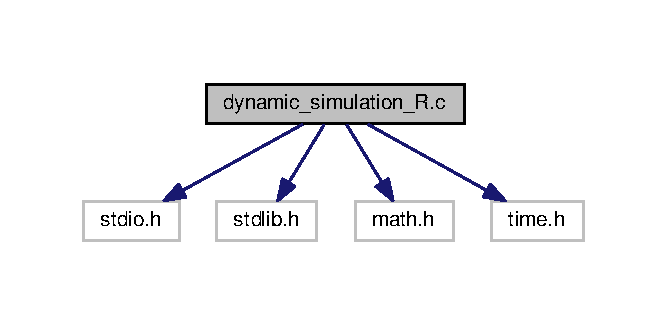
\includegraphics[width=320pt]{d1/d6f/dynamic__simulation__R_8c__incl}
\end{center}
\end{figure}
\subsection*{Functions}
\begin{DoxyCompactItemize}
\item 
int \hyperlink{dynamic__simulation__R_8c_afba1b700b4f80dc7fe8f5a059e8e41d1}{choose\+\_\+ra\+\_\+ru} (int sta\+\_\+1, int tt)
\begin{DoxyCompactList}\small\item\em for performimg backoff, select R\+A-\/\+RU, and check collision \end{DoxyCompactList}\item 
int \hyperlink{dynamic__simulation__R_8c_ae66f6b31b5ad750f1fe042a706a4e3d4}{main} ()
\begin{DoxyCompactList}\small\item\em main function and calculate the performance metrics \end{DoxyCompactList}\end{DoxyCompactItemize}
\subsection*{Variables}
\begin{DoxyCompactItemize}
\item 
int \hyperlink{dynamic__simulation__R_8c_ab2cb8ab426f06c27553b10c73a4f795c}{sta} = 10
\begin{DoxyCompactList}\small\item\em parameter definition \end{DoxyCompactList}\item 
int \hyperlink{dynamic__simulation__R_8c_a582ad1baf82956c0c42d0570b810b45d}{RU} = 15
\begin{DoxyCompactList}\small\item\em number of RU \end{DoxyCompactList}\item 
int \hyperlink{dynamic__simulation__R_8c_a66220f2712ab879767e2b0b1f3e79c1d}{Lmax} = 5
\begin{DoxyCompactList}\small\item\em retry limit \end{DoxyCompactList}\item 
float \hyperlink{dynamic__simulation__R_8c_af540ad79fc6f6f86be9d1ed30d10f327}{dynamic\+\_\+\+RU} \mbox{[}80\mbox{]}
\begin{DoxyCompactList}\small\item\em number of R\+A-\/\+RU in each slot for statistic \end{DoxyCompactList}\item 
int \hyperlink{dynamic__simulation__R_8c_a0a52be688ac0ff37c30d0baffff10c8d}{slot\+\_\+time} = 50
\begin{DoxyCompactList}\small\item\em Imax. \end{DoxyCompactList}\item 
int \hyperlink{dynamic__simulation__R_8c_aab6215b3ec7f291c6cdb9e17912ad805}{packet} = 5
\begin{DoxyCompactList}\small\item\em number of packets pending to transmit \end{DoxyCompactList}\item 
int \hyperlink{dynamic__simulation__R_8c_a510b1e7f30ad20e49970c8cda2c4c530}{packet\+\_\+\+RU} \mbox{[}80\mbox{]} =\{0,15\}
\begin{DoxyCompactList}\small\item\em number of R\+A-\/\+RU in each slot \end{DoxyCompactList}\item 
int \hyperlink{dynamic__simulation__R_8c_a5a0647044878596436db4807d9c76382}{success\+\_\+sta}
\begin{DoxyCompactList}\small\item\em number of success S\+TA for statistic \end{DoxyCompactList}\item 
int \hyperlink{dynamic__simulation__R_8c_a8983b76586c41a8e1af2aaae1d879d64}{total\+\_\+success\+\_\+sta}
\item 
int \hyperlink{dynamic__simulation__R_8c_aa61eed7630095c964ee884133cfd51be}{select\+\_\+ra\+\_\+ru}
\begin{DoxyCompactList}\small\item\em number of R\+A-\/\+RU select by S\+TA \end{DoxyCompactList}\item 
int \hyperlink{dynamic__simulation__R_8c_a685d345363a9d2c46bf5aacf43807109}{usable\+\_\+ra\+\_\+ru}
\begin{DoxyCompactList}\small\item\em for calculating the number of R\+A-\/\+RU in each slot \end{DoxyCompactList}\item 
int \hyperlink{dynamic__simulation__R_8c_a68eaf9a59ffba031bf1dc152e3b023e0}{fail}
\begin{DoxyCompactList}\small\item\em number of failed S\+TA \end{DoxyCompactList}\item 
int \hyperlink{dynamic__simulation__R_8c_a3494600bf5984023e0bea4c64a0a26f3}{backoff}
\begin{DoxyCompactList}\small\item\em O\+BO counter. \end{DoxyCompactList}\item 
int \hyperlink{dynamic__simulation__R_8c_a1bd3f5fbccb1628eb13dda4cd02633a4}{test}
\begin{DoxyCompactList}\small\item\em the index of for loop of test number \end{DoxyCompactList}\item 
int \hyperlink{dynamic__simulation__R_8c_a1ad9c1fcda5e485d69a60bbcd2eaeb47}{test\+\_\+number} = 100000
\begin{DoxyCompactList}\small\item\em the test number \end{DoxyCompactList}\item 
int \hyperlink{dynamic__simulation__R_8c_afe5cbf9b51e39359f46d1dc7566cc8d6}{check\+\_\+collision} = 99
\item 
int \hyperlink{dynamic__simulation__R_8c_acb559820d9ca11295b4500f179ef6392}{i}
\begin{DoxyCompactList}\small\item\em the index of for loop \end{DoxyCompactList}\item 
int \hyperlink{dynamic__simulation__R_8c_a37d972ae0b47b9099e30983131d31916}{j}
\begin{DoxyCompactList}\small\item\em the index of for loop \end{DoxyCompactList}\item 
int \hyperlink{dynamic__simulation__R_8c_ab66ed8e0098c0a86b458672a55a9cca9}{k}
\begin{DoxyCompactList}\small\item\em the index of for loop \end{DoxyCompactList}\item 
int \hyperlink{dynamic__simulation__R_8c_ac310d9181e916ba43604099aee272c71}{t}
\begin{DoxyCompactList}\small\item\em the index of for loop \end{DoxyCompactList}\item 
int \hyperlink{dynamic__simulation__R_8c_a742204794ea328ba293fe59cec79b990}{m}
\begin{DoxyCompactList}\small\item\em the index of for loop \end{DoxyCompactList}\item 
float \hyperlink{dynamic__simulation__R_8c_abe378c3c05e5a0dc5fa6f312c28418b8}{total\+\_\+cdf}
\begin{DoxyCompactList}\small\item\em the C\+DF for statistic \end{DoxyCompactList}\item 
float \hyperlink{dynamic__simulation__R_8c_a43a06ba231e62d42dc94e15a9e4c2ab9}{test\+\_\+cdf}
\begin{DoxyCompactList}\small\item\em the C\+DF for statistic \end{DoxyCompactList}\item 
float \hyperlink{dynamic__simulation__R_8c_ae9657099ad469924f51cfefe0064e585}{access\+\_\+delay}
\begin{DoxyCompactList}\small\item\em the average access delay for statistic \end{DoxyCompactList}\item 
float \hyperlink{dynamic__simulation__R_8c_ae47e7fad657dc35075edcfd37657504d}{test\+\_\+access\+\_\+delay}
\begin{DoxyCompactList}\small\item\em the average access delay for statistic \end{DoxyCompactList}\item 
float \hyperlink{dynamic__simulation__R_8c_a61b1340a95b065b69db7a2d59c20639e}{first\+\_\+access\+\_\+delay}
\begin{DoxyCompactList}\small\item\em the average access delay for statistic \end{DoxyCompactList}\item 
float \hyperlink{dynamic__simulation__R_8c_a45405f028a24aca07edbdc86f1d5f393}{total\+\_\+access\+\_\+delay}
\begin{DoxyCompactList}\small\item\em the average access delay for statistic \end{DoxyCompactList}\item 
int \hyperlink{dynamic__simulation__R_8c_aa10f3ce8ce2725bf282ddf8ee517ef9e}{S\+TA} \mbox{[}101\mbox{]}\mbox{[}3\mbox{]}
\begin{DoxyCompactList}\small\item\em S\+TA\mbox{[} \mbox{]}\mbox{[}0\mbox{]}\+:Lmax, S\+TA\mbox{[} \mbox{]}\mbox{[}1\mbox{]}\+:O\+BO, S\+TA\mbox{[} \mbox{]}\mbox{[}2\mbox{]}\+:the times of occupying R\+A-\/\+RU. \end{DoxyCompactList}\item 
int \hyperlink{dynamic__simulation__R_8c_acdcce33ff79b661366a072bc6e40c02c}{N\+E\+W\+\_\+\+S\+TA} \mbox{[}101\mbox{]}\mbox{[}2\mbox{]}
\item 
int \hyperlink{dynamic__simulation__R_8c_a5d0ed336c8c3f1d945abbb8dbbe07560}{R\+A\+\_\+\+RU} \mbox{[}15\mbox{]}\mbox{[}100\mbox{]}
\item 
int \hyperlink{dynamic__simulation__R_8c_ada1afa9a53388da4a95940fd11dd92ae}{Fm} \mbox{[}6\mbox{]}
\item 
int \hyperlink{dynamic__simulation__R_8c_ad459e9aac25af28f98af039ef042d25d}{total\+\_\+\+Fm} \mbox{[}6\mbox{]}
\item 
float \hyperlink{dynamic__simulation__R_8c_a5f504685acdd057d7031ffe41859b516}{M\+\_\+i\+\_\+s} \mbox{[}80\mbox{]}\mbox{[}6\mbox{]}
\begin{DoxyCompactList}\small\item\em the number of success S\+TA in each slot \end{DoxyCompactList}\item 
float \hyperlink{dynamic__simulation__R_8c_a1c317864f6e20f7b81d080a052a2a548}{M\+\_\+i\+\_\+s\+\_\+for\+\_\+time} \mbox{[}80\mbox{]}
\begin{DoxyCompactList}\small\item\em the number of success S\+TA in each slot \end{DoxyCompactList}\item 
float \hyperlink{dynamic__simulation__R_8c_a8ddb29de6cbe5dbcac983fa75b5180d3}{s\+\_\+packet} \mbox{[}80\mbox{]}
\item 
float \hyperlink{dynamic__simulation__R_8c_acec638afeb56200b7d2ca21dcb7ba00b}{M\+\_\+i\+\_\+f} \mbox{[}80\mbox{]}\mbox{[}6\mbox{]}
\begin{DoxyCompactList}\small\item\em the number of failed S\+TA in each slot \end{DoxyCompactList}\item 
float \hyperlink{dynamic__simulation__R_8c_aeee3833115dd3264acf2461340c56525}{M\+\_\+i\+\_\+f\+\_\+for\+\_\+time} \mbox{[}80\mbox{]}
\begin{DoxyCompactList}\small\item\em the number of failed S\+TA in each slot \end{DoxyCompactList}\item 
float \hyperlink{dynamic__simulation__R_8c_a0553d0e70bca3c413f6eef1c18f5431f}{M\+\_\+i\+\_\+for\+\_\+time} \mbox{[}80\mbox{]}
\begin{DoxyCompactList}\small\item\em the number of contending S\+TA in each slot \end{DoxyCompactList}\item 
float \hyperlink{dynamic__simulation__R_8c_a6a5676e2a29f2b90511009d887b4091a}{success\+\_\+packet}
\begin{DoxyCompactList}\small\item\em the access success probability for packet for statistic \end{DoxyCompactList}\item 
float \hyperlink{dynamic__simulation__R_8c_a9bfb2687ec98c3ee1596ab570c68506a}{total\+\_\+success\+\_\+packet}
\begin{DoxyCompactList}\small\item\em the access success probability for packet for statistic \end{DoxyCompactList}\item 
float \hyperlink{dynamic__simulation__R_8c_a7046ea24990cf1c7b54383f96dd10735}{test\+\_\+success\+\_\+packet}
\begin{DoxyCompactList}\small\item\em the access success probability for packet for statistic \end{DoxyCompactList}\item 
float \hyperlink{dynamic__simulation__R_8c_ab11708df5cbd77e863d800392df5408e}{test\+\_\+success\+\_\+packet\+\_\+probability}
\begin{DoxyCompactList}\small\item\em the access success probability for packet for statistic \end{DoxyCompactList}\item 
float \hyperlink{dynamic__simulation__R_8c_ad93274f2b64c938cd4fade99d2bcf781}{test\+\_\+success\+\_\+probability}
\begin{DoxyCompactList}\small\item\em the access success probability for S\+TA for statistic \end{DoxyCompactList}\item 
float \hyperlink{dynamic__simulation__R_8c_acb9872e8a780d9792317255be909fe22}{success\+\_\+probability}
\begin{DoxyCompactList}\small\item\em the access success probability for S\+TA for statistic \end{DoxyCompactList}\end{DoxyCompactItemize}


\subsection{Function Documentation}
\index{dynamic\+\_\+simulation\+\_\+\+R.\+c@{dynamic\+\_\+simulation\+\_\+\+R.\+c}!choose\+\_\+ra\+\_\+ru@{choose\+\_\+ra\+\_\+ru}}
\index{choose\+\_\+ra\+\_\+ru@{choose\+\_\+ra\+\_\+ru}!dynamic\+\_\+simulation\+\_\+\+R.\+c@{dynamic\+\_\+simulation\+\_\+\+R.\+c}}
\subsubsection[{\texorpdfstring{choose\+\_\+ra\+\_\+ru(int sta\+\_\+1, int tt)}{choose_ra_ru(int sta_1, int tt)}}]{\setlength{\rightskip}{0pt plus 5cm}int choose\+\_\+ra\+\_\+ru (
\begin{DoxyParamCaption}
\item[{int}]{sta\+\_\+1, }
\item[{int}]{tt}
\end{DoxyParamCaption}
)}\hypertarget{dynamic__simulation__R_8c_afba1b700b4f80dc7fe8f5a059e8e41d1}{}\label{dynamic__simulation__R_8c_afba1b700b4f80dc7fe8f5a059e8e41d1}


for performimg backoff, select R\+A-\/\+RU, and check collision 

dynamic RU

pre-\/backoff

O\+C\+Wmin

backoff number -\/ RU

select a RU randomly

contention time+1

contention times$>$Lmax, leave this loop

fill the S\+TA in the array of R\+A-\/\+RU

keep the backoff number

check collision of R\+A-\/\+RU

the times of occupying the R\+A-\/\+RU

success packet

the occupying RU=1, the non-\/occupying RU=0

calculate the number of success sta and C\+DF

C\+DF

remove the backoff number from the success S\+TA

when counter $>$ the number of packet, release this RU

remove the S\+TA index from the success S\+TA

release the occupying R\+A-\/\+RU

the occupying RU=1, the non-\/occupying RU=0 

References backoff, check\+\_\+collision, fail, Fm, i, j, k, Lmax, m, M\+\_\+i\+\_\+f, M\+\_\+i\+\_\+f\+\_\+for\+\_\+time, M\+\_\+i\+\_\+s, N\+E\+W\+\_\+\+S\+TA, packet, packet\+\_\+\+RU, R\+A\+\_\+\+RU, select\+\_\+ra\+\_\+ru, S\+TA, success\+\_\+packet, success\+\_\+sta, and usable\+\_\+ra\+\_\+ru.



Referenced by main().

\index{dynamic\+\_\+simulation\+\_\+\+R.\+c@{dynamic\+\_\+simulation\+\_\+\+R.\+c}!main@{main}}
\index{main@{main}!dynamic\+\_\+simulation\+\_\+\+R.\+c@{dynamic\+\_\+simulation\+\_\+\+R.\+c}}
\subsubsection[{\texorpdfstring{main()}{main()}}]{\setlength{\rightskip}{0pt plus 5cm}int main (
\begin{DoxyParamCaption}
{}
\end{DoxyParamCaption}
)}\hypertarget{dynamic__simulation__R_8c_ae66f6b31b5ad750f1fe042a706a4e3d4}{}\label{dynamic__simulation__R_8c_ae66f6b31b5ad750f1fe042a706a4e3d4}


main function and calculate the performance metrics 

success sta

success packet

access delay

Ri

average access delay

access success probability

success packet

success packet probability

C\+DF

i v.\+s. M\+\_\+i,s\mbox{[}n\mbox{]} 

References access\+\_\+delay, choose\+\_\+ra\+\_\+ru(), dynamic\+\_\+\+RU, fail, first\+\_\+access\+\_\+delay, Fm, i, Lmax, m, M\+\_\+i\+\_\+f, M\+\_\+i\+\_\+f\+\_\+for\+\_\+time, M\+\_\+i\+\_\+s, M\+\_\+i\+\_\+s\+\_\+for\+\_\+time, N\+E\+W\+\_\+\+S\+TA, packet, packet\+\_\+\+RU, R\+A\+\_\+\+RU, slot\+\_\+time, sta, S\+TA, success\+\_\+packet, success\+\_\+sta, t, test, test\+\_\+access\+\_\+delay, test\+\_\+cdf, test\+\_\+number, test\+\_\+success\+\_\+packet, test\+\_\+success\+\_\+packet\+\_\+probability, test\+\_\+success\+\_\+probability, total\+\_\+access\+\_\+delay, total\+\_\+cdf, total\+\_\+success\+\_\+packet, total\+\_\+success\+\_\+sta, and usable\+\_\+ra\+\_\+ru.



Here is the call graph for this function\+:\nopagebreak
\begin{figure}[H]
\begin{center}
\leavevmode
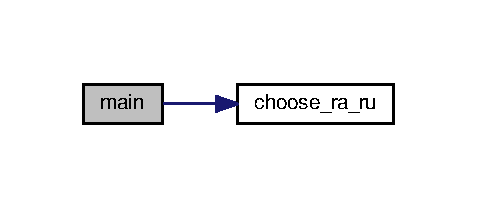
\includegraphics[width=229pt]{d2/d2a/dynamic__simulation__R_8c_ae66f6b31b5ad750f1fe042a706a4e3d4_cgraph}
\end{center}
\end{figure}




\subsection{Variable Documentation}
\index{dynamic\+\_\+simulation\+\_\+\+R.\+c@{dynamic\+\_\+simulation\+\_\+\+R.\+c}!access\+\_\+delay@{access\+\_\+delay}}
\index{access\+\_\+delay@{access\+\_\+delay}!dynamic\+\_\+simulation\+\_\+\+R.\+c@{dynamic\+\_\+simulation\+\_\+\+R.\+c}}
\subsubsection[{\texorpdfstring{access\+\_\+delay}{access_delay}}]{\setlength{\rightskip}{0pt plus 5cm}float access\+\_\+delay}\hypertarget{dynamic__simulation__R_8c_ae9657099ad469924f51cfefe0064e585}{}\label{dynamic__simulation__R_8c_ae9657099ad469924f51cfefe0064e585}


the average access delay for statistic 



Referenced by main().

\index{dynamic\+\_\+simulation\+\_\+\+R.\+c@{dynamic\+\_\+simulation\+\_\+\+R.\+c}!backoff@{backoff}}
\index{backoff@{backoff}!dynamic\+\_\+simulation\+\_\+\+R.\+c@{dynamic\+\_\+simulation\+\_\+\+R.\+c}}
\subsubsection[{\texorpdfstring{backoff}{backoff}}]{\setlength{\rightskip}{0pt plus 5cm}int backoff}\hypertarget{dynamic__simulation__R_8c_a3494600bf5984023e0bea4c64a0a26f3}{}\label{dynamic__simulation__R_8c_a3494600bf5984023e0bea4c64a0a26f3}


O\+BO counter. 



Referenced by choose\+\_\+ra\+\_\+ru().

\index{dynamic\+\_\+simulation\+\_\+\+R.\+c@{dynamic\+\_\+simulation\+\_\+\+R.\+c}!check\+\_\+collision@{check\+\_\+collision}}
\index{check\+\_\+collision@{check\+\_\+collision}!dynamic\+\_\+simulation\+\_\+\+R.\+c@{dynamic\+\_\+simulation\+\_\+\+R.\+c}}
\subsubsection[{\texorpdfstring{check\+\_\+collision}{check_collision}}]{\setlength{\rightskip}{0pt plus 5cm}int check\+\_\+collision = 99}\hypertarget{dynamic__simulation__R_8c_afe5cbf9b51e39359f46d1dc7566cc8d6}{}\label{dynamic__simulation__R_8c_afe5cbf9b51e39359f46d1dc7566cc8d6}


Referenced by choose\+\_\+ra\+\_\+ru().

\index{dynamic\+\_\+simulation\+\_\+\+R.\+c@{dynamic\+\_\+simulation\+\_\+\+R.\+c}!dynamic\+\_\+\+RU@{dynamic\+\_\+\+RU}}
\index{dynamic\+\_\+\+RU@{dynamic\+\_\+\+RU}!dynamic\+\_\+simulation\+\_\+\+R.\+c@{dynamic\+\_\+simulation\+\_\+\+R.\+c}}
\subsubsection[{\texorpdfstring{dynamic\+\_\+\+RU}{dynamic_RU}}]{\setlength{\rightskip}{0pt plus 5cm}float dynamic\+\_\+\+RU\mbox{[}80\mbox{]}}\hypertarget{dynamic__simulation__R_8c_af540ad79fc6f6f86be9d1ed30d10f327}{}\label{dynamic__simulation__R_8c_af540ad79fc6f6f86be9d1ed30d10f327}


number of R\+A-\/\+RU in each slot for statistic 



Referenced by main().

\index{dynamic\+\_\+simulation\+\_\+\+R.\+c@{dynamic\+\_\+simulation\+\_\+\+R.\+c}!fail@{fail}}
\index{fail@{fail}!dynamic\+\_\+simulation\+\_\+\+R.\+c@{dynamic\+\_\+simulation\+\_\+\+R.\+c}}
\subsubsection[{\texorpdfstring{fail}{fail}}]{\setlength{\rightskip}{0pt plus 5cm}int fail}\hypertarget{dynamic__simulation__R_8c_a68eaf9a59ffba031bf1dc152e3b023e0}{}\label{dynamic__simulation__R_8c_a68eaf9a59ffba031bf1dc152e3b023e0}


number of failed S\+TA 



Referenced by choose\+\_\+ra\+\_\+ru(), and main().

\index{dynamic\+\_\+simulation\+\_\+\+R.\+c@{dynamic\+\_\+simulation\+\_\+\+R.\+c}!first\+\_\+access\+\_\+delay@{first\+\_\+access\+\_\+delay}}
\index{first\+\_\+access\+\_\+delay@{first\+\_\+access\+\_\+delay}!dynamic\+\_\+simulation\+\_\+\+R.\+c@{dynamic\+\_\+simulation\+\_\+\+R.\+c}}
\subsubsection[{\texorpdfstring{first\+\_\+access\+\_\+delay}{first_access_delay}}]{\setlength{\rightskip}{0pt plus 5cm}float first\+\_\+access\+\_\+delay}\hypertarget{dynamic__simulation__R_8c_a61b1340a95b065b69db7a2d59c20639e}{}\label{dynamic__simulation__R_8c_a61b1340a95b065b69db7a2d59c20639e}


the average access delay for statistic 



Referenced by main().

\index{dynamic\+\_\+simulation\+\_\+\+R.\+c@{dynamic\+\_\+simulation\+\_\+\+R.\+c}!Fm@{Fm}}
\index{Fm@{Fm}!dynamic\+\_\+simulation\+\_\+\+R.\+c@{dynamic\+\_\+simulation\+\_\+\+R.\+c}}
\subsubsection[{\texorpdfstring{Fm}{Fm}}]{\setlength{\rightskip}{0pt plus 5cm}int Fm\mbox{[}6\mbox{]}}\hypertarget{dynamic__simulation__R_8c_ada1afa9a53388da4a95940fd11dd92ae}{}\label{dynamic__simulation__R_8c_ada1afa9a53388da4a95940fd11dd92ae}


Referenced by choose\+\_\+ra\+\_\+ru(), and main().

\index{dynamic\+\_\+simulation\+\_\+\+R.\+c@{dynamic\+\_\+simulation\+\_\+\+R.\+c}!i@{i}}
\index{i@{i}!dynamic\+\_\+simulation\+\_\+\+R.\+c@{dynamic\+\_\+simulation\+\_\+\+R.\+c}}
\subsubsection[{\texorpdfstring{i}{i}}]{\setlength{\rightskip}{0pt plus 5cm}int i}\hypertarget{dynamic__simulation__R_8c_acb559820d9ca11295b4500f179ef6392}{}\label{dynamic__simulation__R_8c_acb559820d9ca11295b4500f179ef6392}


the index of for loop 



Referenced by choose\+\_\+ra\+\_\+ru(), and main().

\index{dynamic\+\_\+simulation\+\_\+\+R.\+c@{dynamic\+\_\+simulation\+\_\+\+R.\+c}!j@{j}}
\index{j@{j}!dynamic\+\_\+simulation\+\_\+\+R.\+c@{dynamic\+\_\+simulation\+\_\+\+R.\+c}}
\subsubsection[{\texorpdfstring{j}{j}}]{\setlength{\rightskip}{0pt plus 5cm}int j}\hypertarget{dynamic__simulation__R_8c_a37d972ae0b47b9099e30983131d31916}{}\label{dynamic__simulation__R_8c_a37d972ae0b47b9099e30983131d31916}


the index of for loop 



Referenced by choose\+\_\+ra\+\_\+ru().

\index{dynamic\+\_\+simulation\+\_\+\+R.\+c@{dynamic\+\_\+simulation\+\_\+\+R.\+c}!k@{k}}
\index{k@{k}!dynamic\+\_\+simulation\+\_\+\+R.\+c@{dynamic\+\_\+simulation\+\_\+\+R.\+c}}
\subsubsection[{\texorpdfstring{k}{k}}]{\setlength{\rightskip}{0pt plus 5cm}int k}\hypertarget{dynamic__simulation__R_8c_ab66ed8e0098c0a86b458672a55a9cca9}{}\label{dynamic__simulation__R_8c_ab66ed8e0098c0a86b458672a55a9cca9}


the index of for loop 



Referenced by choose\+\_\+ra\+\_\+ru().

\index{dynamic\+\_\+simulation\+\_\+\+R.\+c@{dynamic\+\_\+simulation\+\_\+\+R.\+c}!Lmax@{Lmax}}
\index{Lmax@{Lmax}!dynamic\+\_\+simulation\+\_\+\+R.\+c@{dynamic\+\_\+simulation\+\_\+\+R.\+c}}
\subsubsection[{\texorpdfstring{Lmax}{Lmax}}]{\setlength{\rightskip}{0pt plus 5cm}int Lmax = 5}\hypertarget{dynamic__simulation__R_8c_a66220f2712ab879767e2b0b1f3e79c1d}{}\label{dynamic__simulation__R_8c_a66220f2712ab879767e2b0b1f3e79c1d}


retry limit 



Referenced by choose\+\_\+ra\+\_\+ru(), and main().

\index{dynamic\+\_\+simulation\+\_\+\+R.\+c@{dynamic\+\_\+simulation\+\_\+\+R.\+c}!m@{m}}
\index{m@{m}!dynamic\+\_\+simulation\+\_\+\+R.\+c@{dynamic\+\_\+simulation\+\_\+\+R.\+c}}
\subsubsection[{\texorpdfstring{m}{m}}]{\setlength{\rightskip}{0pt plus 5cm}int m}\hypertarget{dynamic__simulation__R_8c_a742204794ea328ba293fe59cec79b990}{}\label{dynamic__simulation__R_8c_a742204794ea328ba293fe59cec79b990}


the index of for loop 



Referenced by choose\+\_\+ra\+\_\+ru(), and main().

\index{dynamic\+\_\+simulation\+\_\+\+R.\+c@{dynamic\+\_\+simulation\+\_\+\+R.\+c}!M\+\_\+i\+\_\+f@{M\+\_\+i\+\_\+f}}
\index{M\+\_\+i\+\_\+f@{M\+\_\+i\+\_\+f}!dynamic\+\_\+simulation\+\_\+\+R.\+c@{dynamic\+\_\+simulation\+\_\+\+R.\+c}}
\subsubsection[{\texorpdfstring{M\+\_\+i\+\_\+f}{M_i_f}}]{\setlength{\rightskip}{0pt plus 5cm}float M\+\_\+i\+\_\+f\mbox{[}80\mbox{]}\mbox{[}6\mbox{]}}\hypertarget{dynamic__simulation__R_8c_acec638afeb56200b7d2ca21dcb7ba00b}{}\label{dynamic__simulation__R_8c_acec638afeb56200b7d2ca21dcb7ba00b}


the number of failed S\+TA in each slot 



Referenced by choose\+\_\+ra\+\_\+ru(), and main().

\index{dynamic\+\_\+simulation\+\_\+\+R.\+c@{dynamic\+\_\+simulation\+\_\+\+R.\+c}!M\+\_\+i\+\_\+f\+\_\+for\+\_\+time@{M\+\_\+i\+\_\+f\+\_\+for\+\_\+time}}
\index{M\+\_\+i\+\_\+f\+\_\+for\+\_\+time@{M\+\_\+i\+\_\+f\+\_\+for\+\_\+time}!dynamic\+\_\+simulation\+\_\+\+R.\+c@{dynamic\+\_\+simulation\+\_\+\+R.\+c}}
\subsubsection[{\texorpdfstring{M\+\_\+i\+\_\+f\+\_\+for\+\_\+time}{M_i_f_for_time}}]{\setlength{\rightskip}{0pt plus 5cm}float M\+\_\+i\+\_\+f\+\_\+for\+\_\+time\mbox{[}80\mbox{]}}\hypertarget{dynamic__simulation__R_8c_aeee3833115dd3264acf2461340c56525}{}\label{dynamic__simulation__R_8c_aeee3833115dd3264acf2461340c56525}


the number of failed S\+TA in each slot 



Referenced by choose\+\_\+ra\+\_\+ru(), and main().

\index{dynamic\+\_\+simulation\+\_\+\+R.\+c@{dynamic\+\_\+simulation\+\_\+\+R.\+c}!M\+\_\+i\+\_\+for\+\_\+time@{M\+\_\+i\+\_\+for\+\_\+time}}
\index{M\+\_\+i\+\_\+for\+\_\+time@{M\+\_\+i\+\_\+for\+\_\+time}!dynamic\+\_\+simulation\+\_\+\+R.\+c@{dynamic\+\_\+simulation\+\_\+\+R.\+c}}
\subsubsection[{\texorpdfstring{M\+\_\+i\+\_\+for\+\_\+time}{M_i_for_time}}]{\setlength{\rightskip}{0pt plus 5cm}float M\+\_\+i\+\_\+for\+\_\+time\mbox{[}80\mbox{]}}\hypertarget{dynamic__simulation__R_8c_a0553d0e70bca3c413f6eef1c18f5431f}{}\label{dynamic__simulation__R_8c_a0553d0e70bca3c413f6eef1c18f5431f}


the number of contending S\+TA in each slot 

\index{dynamic\+\_\+simulation\+\_\+\+R.\+c@{dynamic\+\_\+simulation\+\_\+\+R.\+c}!M\+\_\+i\+\_\+s@{M\+\_\+i\+\_\+s}}
\index{M\+\_\+i\+\_\+s@{M\+\_\+i\+\_\+s}!dynamic\+\_\+simulation\+\_\+\+R.\+c@{dynamic\+\_\+simulation\+\_\+\+R.\+c}}
\subsubsection[{\texorpdfstring{M\+\_\+i\+\_\+s}{M_i_s}}]{\setlength{\rightskip}{0pt plus 5cm}float M\+\_\+i\+\_\+s\mbox{[}80\mbox{]}\mbox{[}6\mbox{]}}\hypertarget{dynamic__simulation__R_8c_a5f504685acdd057d7031ffe41859b516}{}\label{dynamic__simulation__R_8c_a5f504685acdd057d7031ffe41859b516}


the number of success S\+TA in each slot 



Referenced by choose\+\_\+ra\+\_\+ru(), and main().

\index{dynamic\+\_\+simulation\+\_\+\+R.\+c@{dynamic\+\_\+simulation\+\_\+\+R.\+c}!M\+\_\+i\+\_\+s\+\_\+for\+\_\+time@{M\+\_\+i\+\_\+s\+\_\+for\+\_\+time}}
\index{M\+\_\+i\+\_\+s\+\_\+for\+\_\+time@{M\+\_\+i\+\_\+s\+\_\+for\+\_\+time}!dynamic\+\_\+simulation\+\_\+\+R.\+c@{dynamic\+\_\+simulation\+\_\+\+R.\+c}}
\subsubsection[{\texorpdfstring{M\+\_\+i\+\_\+s\+\_\+for\+\_\+time}{M_i_s_for_time}}]{\setlength{\rightskip}{0pt plus 5cm}float M\+\_\+i\+\_\+s\+\_\+for\+\_\+time\mbox{[}80\mbox{]}}\hypertarget{dynamic__simulation__R_8c_a1c317864f6e20f7b81d080a052a2a548}{}\label{dynamic__simulation__R_8c_a1c317864f6e20f7b81d080a052a2a548}


the number of success S\+TA in each slot 



Referenced by main().

\index{dynamic\+\_\+simulation\+\_\+\+R.\+c@{dynamic\+\_\+simulation\+\_\+\+R.\+c}!N\+E\+W\+\_\+\+S\+TA@{N\+E\+W\+\_\+\+S\+TA}}
\index{N\+E\+W\+\_\+\+S\+TA@{N\+E\+W\+\_\+\+S\+TA}!dynamic\+\_\+simulation\+\_\+\+R.\+c@{dynamic\+\_\+simulation\+\_\+\+R.\+c}}
\subsubsection[{\texorpdfstring{N\+E\+W\+\_\+\+S\+TA}{NEW_STA}}]{\setlength{\rightskip}{0pt plus 5cm}int N\+E\+W\+\_\+\+S\+TA\mbox{[}101\mbox{]}\mbox{[}2\mbox{]}}\hypertarget{dynamic__simulation__R_8c_acdcce33ff79b661366a072bc6e40c02c}{}\label{dynamic__simulation__R_8c_acdcce33ff79b661366a072bc6e40c02c}


Referenced by choose\+\_\+ra\+\_\+ru(), and main().

\index{dynamic\+\_\+simulation\+\_\+\+R.\+c@{dynamic\+\_\+simulation\+\_\+\+R.\+c}!packet@{packet}}
\index{packet@{packet}!dynamic\+\_\+simulation\+\_\+\+R.\+c@{dynamic\+\_\+simulation\+\_\+\+R.\+c}}
\subsubsection[{\texorpdfstring{packet}{packet}}]{\setlength{\rightskip}{0pt plus 5cm}int packet = 5}\hypertarget{dynamic__simulation__R_8c_aab6215b3ec7f291c6cdb9e17912ad805}{}\label{dynamic__simulation__R_8c_aab6215b3ec7f291c6cdb9e17912ad805}


number of packets pending to transmit 



Referenced by choose\+\_\+ra\+\_\+ru(), and main().

\index{dynamic\+\_\+simulation\+\_\+\+R.\+c@{dynamic\+\_\+simulation\+\_\+\+R.\+c}!packet\+\_\+\+RU@{packet\+\_\+\+RU}}
\index{packet\+\_\+\+RU@{packet\+\_\+\+RU}!dynamic\+\_\+simulation\+\_\+\+R.\+c@{dynamic\+\_\+simulation\+\_\+\+R.\+c}}
\subsubsection[{\texorpdfstring{packet\+\_\+\+RU}{packet_RU}}]{\setlength{\rightskip}{0pt plus 5cm}int packet\+\_\+\+RU\mbox{[}80\mbox{]} =\{0,15\}}\hypertarget{dynamic__simulation__R_8c_a510b1e7f30ad20e49970c8cda2c4c530}{}\label{dynamic__simulation__R_8c_a510b1e7f30ad20e49970c8cda2c4c530}


number of R\+A-\/\+RU in each slot 



Referenced by choose\+\_\+ra\+\_\+ru(), and main().

\index{dynamic\+\_\+simulation\+\_\+\+R.\+c@{dynamic\+\_\+simulation\+\_\+\+R.\+c}!R\+A\+\_\+\+RU@{R\+A\+\_\+\+RU}}
\index{R\+A\+\_\+\+RU@{R\+A\+\_\+\+RU}!dynamic\+\_\+simulation\+\_\+\+R.\+c@{dynamic\+\_\+simulation\+\_\+\+R.\+c}}
\subsubsection[{\texorpdfstring{R\+A\+\_\+\+RU}{RA_RU}}]{\setlength{\rightskip}{0pt plus 5cm}int R\+A\+\_\+\+RU\mbox{[}15\mbox{]}\mbox{[}100\mbox{]}}\hypertarget{dynamic__simulation__R_8c_a5d0ed336c8c3f1d945abbb8dbbe07560}{}\label{dynamic__simulation__R_8c_a5d0ed336c8c3f1d945abbb8dbbe07560}


Referenced by choose\+\_\+ra\+\_\+ru(), and main().

\index{dynamic\+\_\+simulation\+\_\+\+R.\+c@{dynamic\+\_\+simulation\+\_\+\+R.\+c}!RU@{RU}}
\index{RU@{RU}!dynamic\+\_\+simulation\+\_\+\+R.\+c@{dynamic\+\_\+simulation\+\_\+\+R.\+c}}
\subsubsection[{\texorpdfstring{RU}{RU}}]{\setlength{\rightskip}{0pt plus 5cm}int RU = 15}\hypertarget{dynamic__simulation__R_8c_a582ad1baf82956c0c42d0570b810b45d}{}\label{dynamic__simulation__R_8c_a582ad1baf82956c0c42d0570b810b45d}


number of RU 

\index{dynamic\+\_\+simulation\+\_\+\+R.\+c@{dynamic\+\_\+simulation\+\_\+\+R.\+c}!s\+\_\+packet@{s\+\_\+packet}}
\index{s\+\_\+packet@{s\+\_\+packet}!dynamic\+\_\+simulation\+\_\+\+R.\+c@{dynamic\+\_\+simulation\+\_\+\+R.\+c}}
\subsubsection[{\texorpdfstring{s\+\_\+packet}{s_packet}}]{\setlength{\rightskip}{0pt plus 5cm}float s\+\_\+packet\mbox{[}80\mbox{]}}\hypertarget{dynamic__simulation__R_8c_a8ddb29de6cbe5dbcac983fa75b5180d3}{}\label{dynamic__simulation__R_8c_a8ddb29de6cbe5dbcac983fa75b5180d3}
\index{dynamic\+\_\+simulation\+\_\+\+R.\+c@{dynamic\+\_\+simulation\+\_\+\+R.\+c}!select\+\_\+ra\+\_\+ru@{select\+\_\+ra\+\_\+ru}}
\index{select\+\_\+ra\+\_\+ru@{select\+\_\+ra\+\_\+ru}!dynamic\+\_\+simulation\+\_\+\+R.\+c@{dynamic\+\_\+simulation\+\_\+\+R.\+c}}
\subsubsection[{\texorpdfstring{select\+\_\+ra\+\_\+ru}{select_ra_ru}}]{\setlength{\rightskip}{0pt plus 5cm}int select\+\_\+ra\+\_\+ru}\hypertarget{dynamic__simulation__R_8c_aa61eed7630095c964ee884133cfd51be}{}\label{dynamic__simulation__R_8c_aa61eed7630095c964ee884133cfd51be}


number of R\+A-\/\+RU select by S\+TA 



Referenced by choose\+\_\+ra\+\_\+ru().

\index{dynamic\+\_\+simulation\+\_\+\+R.\+c@{dynamic\+\_\+simulation\+\_\+\+R.\+c}!slot\+\_\+time@{slot\+\_\+time}}
\index{slot\+\_\+time@{slot\+\_\+time}!dynamic\+\_\+simulation\+\_\+\+R.\+c@{dynamic\+\_\+simulation\+\_\+\+R.\+c}}
\subsubsection[{\texorpdfstring{slot\+\_\+time}{slot_time}}]{\setlength{\rightskip}{0pt plus 5cm}int slot\+\_\+time = 50}\hypertarget{dynamic__simulation__R_8c_a0a52be688ac0ff37c30d0baffff10c8d}{}\label{dynamic__simulation__R_8c_a0a52be688ac0ff37c30d0baffff10c8d}


Imax. 



Referenced by main().

\index{dynamic\+\_\+simulation\+\_\+\+R.\+c@{dynamic\+\_\+simulation\+\_\+\+R.\+c}!sta@{sta}}
\index{sta@{sta}!dynamic\+\_\+simulation\+\_\+\+R.\+c@{dynamic\+\_\+simulation\+\_\+\+R.\+c}}
\subsubsection[{\texorpdfstring{sta}{sta}}]{\setlength{\rightskip}{0pt plus 5cm}int sta = 10}\hypertarget{dynamic__simulation__R_8c_ab2cb8ab426f06c27553b10c73a4f795c}{}\label{dynamic__simulation__R_8c_ab2cb8ab426f06c27553b10c73a4f795c}


parameter definition 

total S\+TA number 

Referenced by main().

\index{dynamic\+\_\+simulation\+\_\+\+R.\+c@{dynamic\+\_\+simulation\+\_\+\+R.\+c}!S\+TA@{S\+TA}}
\index{S\+TA@{S\+TA}!dynamic\+\_\+simulation\+\_\+\+R.\+c@{dynamic\+\_\+simulation\+\_\+\+R.\+c}}
\subsubsection[{\texorpdfstring{S\+TA}{STA}}]{\setlength{\rightskip}{0pt plus 5cm}int S\+TA\mbox{[}101\mbox{]}\mbox{[}3\mbox{]}}\hypertarget{dynamic__simulation__R_8c_aa10f3ce8ce2725bf282ddf8ee517ef9e}{}\label{dynamic__simulation__R_8c_aa10f3ce8ce2725bf282ddf8ee517ef9e}


S\+TA\mbox{[} \mbox{]}\mbox{[}0\mbox{]}\+:Lmax, S\+TA\mbox{[} \mbox{]}\mbox{[}1\mbox{]}\+:O\+BO, S\+TA\mbox{[} \mbox{]}\mbox{[}2\mbox{]}\+:the times of occupying R\+A-\/\+RU. 



Referenced by choose\+\_\+ra\+\_\+ru(), and main().

\index{dynamic\+\_\+simulation\+\_\+\+R.\+c@{dynamic\+\_\+simulation\+\_\+\+R.\+c}!success\+\_\+packet@{success\+\_\+packet}}
\index{success\+\_\+packet@{success\+\_\+packet}!dynamic\+\_\+simulation\+\_\+\+R.\+c@{dynamic\+\_\+simulation\+\_\+\+R.\+c}}
\subsubsection[{\texorpdfstring{success\+\_\+packet}{success_packet}}]{\setlength{\rightskip}{0pt plus 5cm}float success\+\_\+packet}\hypertarget{dynamic__simulation__R_8c_a6a5676e2a29f2b90511009d887b4091a}{}\label{dynamic__simulation__R_8c_a6a5676e2a29f2b90511009d887b4091a}


the access success probability for packet for statistic 



Referenced by choose\+\_\+ra\+\_\+ru(), and main().

\index{dynamic\+\_\+simulation\+\_\+\+R.\+c@{dynamic\+\_\+simulation\+\_\+\+R.\+c}!success\+\_\+probability@{success\+\_\+probability}}
\index{success\+\_\+probability@{success\+\_\+probability}!dynamic\+\_\+simulation\+\_\+\+R.\+c@{dynamic\+\_\+simulation\+\_\+\+R.\+c}}
\subsubsection[{\texorpdfstring{success\+\_\+probability}{success_probability}}]{\setlength{\rightskip}{0pt plus 5cm}float success\+\_\+probability}\hypertarget{dynamic__simulation__R_8c_acb9872e8a780d9792317255be909fe22}{}\label{dynamic__simulation__R_8c_acb9872e8a780d9792317255be909fe22}


the access success probability for S\+TA for statistic 

\index{dynamic\+\_\+simulation\+\_\+\+R.\+c@{dynamic\+\_\+simulation\+\_\+\+R.\+c}!success\+\_\+sta@{success\+\_\+sta}}
\index{success\+\_\+sta@{success\+\_\+sta}!dynamic\+\_\+simulation\+\_\+\+R.\+c@{dynamic\+\_\+simulation\+\_\+\+R.\+c}}
\subsubsection[{\texorpdfstring{success\+\_\+sta}{success_sta}}]{\setlength{\rightskip}{0pt plus 5cm}int success\+\_\+sta}\hypertarget{dynamic__simulation__R_8c_a5a0647044878596436db4807d9c76382}{}\label{dynamic__simulation__R_8c_a5a0647044878596436db4807d9c76382}


number of success S\+TA for statistic 



Referenced by choose\+\_\+ra\+\_\+ru(), and main().

\index{dynamic\+\_\+simulation\+\_\+\+R.\+c@{dynamic\+\_\+simulation\+\_\+\+R.\+c}!t@{t}}
\index{t@{t}!dynamic\+\_\+simulation\+\_\+\+R.\+c@{dynamic\+\_\+simulation\+\_\+\+R.\+c}}
\subsubsection[{\texorpdfstring{t}{t}}]{\setlength{\rightskip}{0pt plus 5cm}int t}\hypertarget{dynamic__simulation__R_8c_ac310d9181e916ba43604099aee272c71}{}\label{dynamic__simulation__R_8c_ac310d9181e916ba43604099aee272c71}


the index of for loop 



Referenced by main().

\index{dynamic\+\_\+simulation\+\_\+\+R.\+c@{dynamic\+\_\+simulation\+\_\+\+R.\+c}!test@{test}}
\index{test@{test}!dynamic\+\_\+simulation\+\_\+\+R.\+c@{dynamic\+\_\+simulation\+\_\+\+R.\+c}}
\subsubsection[{\texorpdfstring{test}{test}}]{\setlength{\rightskip}{0pt plus 5cm}int test}\hypertarget{dynamic__simulation__R_8c_a1bd3f5fbccb1628eb13dda4cd02633a4}{}\label{dynamic__simulation__R_8c_a1bd3f5fbccb1628eb13dda4cd02633a4}


the index of for loop of test number 



Referenced by main().

\index{dynamic\+\_\+simulation\+\_\+\+R.\+c@{dynamic\+\_\+simulation\+\_\+\+R.\+c}!test\+\_\+access\+\_\+delay@{test\+\_\+access\+\_\+delay}}
\index{test\+\_\+access\+\_\+delay@{test\+\_\+access\+\_\+delay}!dynamic\+\_\+simulation\+\_\+\+R.\+c@{dynamic\+\_\+simulation\+\_\+\+R.\+c}}
\subsubsection[{\texorpdfstring{test\+\_\+access\+\_\+delay}{test_access_delay}}]{\setlength{\rightskip}{0pt plus 5cm}float test\+\_\+access\+\_\+delay}\hypertarget{dynamic__simulation__R_8c_ae47e7fad657dc35075edcfd37657504d}{}\label{dynamic__simulation__R_8c_ae47e7fad657dc35075edcfd37657504d}


the average access delay for statistic 



Referenced by main().

\index{dynamic\+\_\+simulation\+\_\+\+R.\+c@{dynamic\+\_\+simulation\+\_\+\+R.\+c}!test\+\_\+cdf@{test\+\_\+cdf}}
\index{test\+\_\+cdf@{test\+\_\+cdf}!dynamic\+\_\+simulation\+\_\+\+R.\+c@{dynamic\+\_\+simulation\+\_\+\+R.\+c}}
\subsubsection[{\texorpdfstring{test\+\_\+cdf}{test_cdf}}]{\setlength{\rightskip}{0pt plus 5cm}float test\+\_\+cdf}\hypertarget{dynamic__simulation__R_8c_a43a06ba231e62d42dc94e15a9e4c2ab9}{}\label{dynamic__simulation__R_8c_a43a06ba231e62d42dc94e15a9e4c2ab9}


the C\+DF for statistic 



Referenced by main().

\index{dynamic\+\_\+simulation\+\_\+\+R.\+c@{dynamic\+\_\+simulation\+\_\+\+R.\+c}!test\+\_\+number@{test\+\_\+number}}
\index{test\+\_\+number@{test\+\_\+number}!dynamic\+\_\+simulation\+\_\+\+R.\+c@{dynamic\+\_\+simulation\+\_\+\+R.\+c}}
\subsubsection[{\texorpdfstring{test\+\_\+number}{test_number}}]{\setlength{\rightskip}{0pt plus 5cm}int test\+\_\+number = 100000}\hypertarget{dynamic__simulation__R_8c_a1ad9c1fcda5e485d69a60bbcd2eaeb47}{}\label{dynamic__simulation__R_8c_a1ad9c1fcda5e485d69a60bbcd2eaeb47}


the test number 



Referenced by main().

\index{dynamic\+\_\+simulation\+\_\+\+R.\+c@{dynamic\+\_\+simulation\+\_\+\+R.\+c}!test\+\_\+success\+\_\+packet@{test\+\_\+success\+\_\+packet}}
\index{test\+\_\+success\+\_\+packet@{test\+\_\+success\+\_\+packet}!dynamic\+\_\+simulation\+\_\+\+R.\+c@{dynamic\+\_\+simulation\+\_\+\+R.\+c}}
\subsubsection[{\texorpdfstring{test\+\_\+success\+\_\+packet}{test_success_packet}}]{\setlength{\rightskip}{0pt plus 5cm}float test\+\_\+success\+\_\+packet}\hypertarget{dynamic__simulation__R_8c_a7046ea24990cf1c7b54383f96dd10735}{}\label{dynamic__simulation__R_8c_a7046ea24990cf1c7b54383f96dd10735}


the access success probability for packet for statistic 



Referenced by main().

\index{dynamic\+\_\+simulation\+\_\+\+R.\+c@{dynamic\+\_\+simulation\+\_\+\+R.\+c}!test\+\_\+success\+\_\+packet\+\_\+probability@{test\+\_\+success\+\_\+packet\+\_\+probability}}
\index{test\+\_\+success\+\_\+packet\+\_\+probability@{test\+\_\+success\+\_\+packet\+\_\+probability}!dynamic\+\_\+simulation\+\_\+\+R.\+c@{dynamic\+\_\+simulation\+\_\+\+R.\+c}}
\subsubsection[{\texorpdfstring{test\+\_\+success\+\_\+packet\+\_\+probability}{test_success_packet_probability}}]{\setlength{\rightskip}{0pt plus 5cm}float test\+\_\+success\+\_\+packet\+\_\+probability}\hypertarget{dynamic__simulation__R_8c_ab11708df5cbd77e863d800392df5408e}{}\label{dynamic__simulation__R_8c_ab11708df5cbd77e863d800392df5408e}


the access success probability for packet for statistic 



Referenced by main().

\index{dynamic\+\_\+simulation\+\_\+\+R.\+c@{dynamic\+\_\+simulation\+\_\+\+R.\+c}!test\+\_\+success\+\_\+probability@{test\+\_\+success\+\_\+probability}}
\index{test\+\_\+success\+\_\+probability@{test\+\_\+success\+\_\+probability}!dynamic\+\_\+simulation\+\_\+\+R.\+c@{dynamic\+\_\+simulation\+\_\+\+R.\+c}}
\subsubsection[{\texorpdfstring{test\+\_\+success\+\_\+probability}{test_success_probability}}]{\setlength{\rightskip}{0pt plus 5cm}float test\+\_\+success\+\_\+probability}\hypertarget{dynamic__simulation__R_8c_ad93274f2b64c938cd4fade99d2bcf781}{}\label{dynamic__simulation__R_8c_ad93274f2b64c938cd4fade99d2bcf781}


the access success probability for S\+TA for statistic 



Referenced by main().

\index{dynamic\+\_\+simulation\+\_\+\+R.\+c@{dynamic\+\_\+simulation\+\_\+\+R.\+c}!total\+\_\+access\+\_\+delay@{total\+\_\+access\+\_\+delay}}
\index{total\+\_\+access\+\_\+delay@{total\+\_\+access\+\_\+delay}!dynamic\+\_\+simulation\+\_\+\+R.\+c@{dynamic\+\_\+simulation\+\_\+\+R.\+c}}
\subsubsection[{\texorpdfstring{total\+\_\+access\+\_\+delay}{total_access_delay}}]{\setlength{\rightskip}{0pt plus 5cm}float total\+\_\+access\+\_\+delay}\hypertarget{dynamic__simulation__R_8c_a45405f028a24aca07edbdc86f1d5f393}{}\label{dynamic__simulation__R_8c_a45405f028a24aca07edbdc86f1d5f393}


the average access delay for statistic 



Referenced by main().

\index{dynamic\+\_\+simulation\+\_\+\+R.\+c@{dynamic\+\_\+simulation\+\_\+\+R.\+c}!total\+\_\+cdf@{total\+\_\+cdf}}
\index{total\+\_\+cdf@{total\+\_\+cdf}!dynamic\+\_\+simulation\+\_\+\+R.\+c@{dynamic\+\_\+simulation\+\_\+\+R.\+c}}
\subsubsection[{\texorpdfstring{total\+\_\+cdf}{total_cdf}}]{\setlength{\rightskip}{0pt plus 5cm}float total\+\_\+cdf}\hypertarget{dynamic__simulation__R_8c_abe378c3c05e5a0dc5fa6f312c28418b8}{}\label{dynamic__simulation__R_8c_abe378c3c05e5a0dc5fa6f312c28418b8}


the C\+DF for statistic 



Referenced by main().

\index{dynamic\+\_\+simulation\+\_\+\+R.\+c@{dynamic\+\_\+simulation\+\_\+\+R.\+c}!total\+\_\+\+Fm@{total\+\_\+\+Fm}}
\index{total\+\_\+\+Fm@{total\+\_\+\+Fm}!dynamic\+\_\+simulation\+\_\+\+R.\+c@{dynamic\+\_\+simulation\+\_\+\+R.\+c}}
\subsubsection[{\texorpdfstring{total\+\_\+\+Fm}{total_Fm}}]{\setlength{\rightskip}{0pt plus 5cm}int total\+\_\+\+Fm\mbox{[}6\mbox{]}}\hypertarget{dynamic__simulation__R_8c_ad459e9aac25af28f98af039ef042d25d}{}\label{dynamic__simulation__R_8c_ad459e9aac25af28f98af039ef042d25d}
\index{dynamic\+\_\+simulation\+\_\+\+R.\+c@{dynamic\+\_\+simulation\+\_\+\+R.\+c}!total\+\_\+success\+\_\+packet@{total\+\_\+success\+\_\+packet}}
\index{total\+\_\+success\+\_\+packet@{total\+\_\+success\+\_\+packet}!dynamic\+\_\+simulation\+\_\+\+R.\+c@{dynamic\+\_\+simulation\+\_\+\+R.\+c}}
\subsubsection[{\texorpdfstring{total\+\_\+success\+\_\+packet}{total_success_packet}}]{\setlength{\rightskip}{0pt plus 5cm}float total\+\_\+success\+\_\+packet}\hypertarget{dynamic__simulation__R_8c_a9bfb2687ec98c3ee1596ab570c68506a}{}\label{dynamic__simulation__R_8c_a9bfb2687ec98c3ee1596ab570c68506a}


the access success probability for packet for statistic 



Referenced by main().

\index{dynamic\+\_\+simulation\+\_\+\+R.\+c@{dynamic\+\_\+simulation\+\_\+\+R.\+c}!total\+\_\+success\+\_\+sta@{total\+\_\+success\+\_\+sta}}
\index{total\+\_\+success\+\_\+sta@{total\+\_\+success\+\_\+sta}!dynamic\+\_\+simulation\+\_\+\+R.\+c@{dynamic\+\_\+simulation\+\_\+\+R.\+c}}
\subsubsection[{\texorpdfstring{total\+\_\+success\+\_\+sta}{total_success_sta}}]{\setlength{\rightskip}{0pt plus 5cm}int total\+\_\+success\+\_\+sta}\hypertarget{dynamic__simulation__R_8c_a8983b76586c41a8e1af2aaae1d879d64}{}\label{dynamic__simulation__R_8c_a8983b76586c41a8e1af2aaae1d879d64}


Referenced by main().

\index{dynamic\+\_\+simulation\+\_\+\+R.\+c@{dynamic\+\_\+simulation\+\_\+\+R.\+c}!usable\+\_\+ra\+\_\+ru@{usable\+\_\+ra\+\_\+ru}}
\index{usable\+\_\+ra\+\_\+ru@{usable\+\_\+ra\+\_\+ru}!dynamic\+\_\+simulation\+\_\+\+R.\+c@{dynamic\+\_\+simulation\+\_\+\+R.\+c}}
\subsubsection[{\texorpdfstring{usable\+\_\+ra\+\_\+ru}{usable_ra_ru}}]{\setlength{\rightskip}{0pt plus 5cm}int usable\+\_\+ra\+\_\+ru}\hypertarget{dynamic__simulation__R_8c_a685d345363a9d2c46bf5aacf43807109}{}\label{dynamic__simulation__R_8c_a685d345363a9d2c46bf5aacf43807109}


for calculating the number of R\+A-\/\+RU in each slot 



Referenced by choose\+\_\+ra\+\_\+ru(), and main().


%--- End generated contents ---

% Index
\backmatter
\newpage
\phantomsection
\clearemptydoublepage
\addcontentsline{toc}{chapter}{Index}
\printindex

\end{document}
